%\usepackage{placeins}
%\usepackage{times}
%\usepackage{latexsym}
%\usepackage{amsmath}
%\usepackage{fancyvrb, fancyhdr, theorem, latexsym, color, longtable}
%\usepackage{multirow}
%\usepackage{url}
%\usepackage{bm}
%\usepackage{amssymb}
%
%\usepackage{fixltx2e}
%\usepackage{tabularx}
%\usepackage{hyperref}
%\usepackage{graphicx}
%
%%\usepackage{algorithm}% http://ctan.org/pkg/algorithms
%%\usepackage{algpseudocode}% http://ctan.org/pkg/algorithmicx
%
%%\usepackage[algo2e,lined]{algorithm2e}
%\usepackage{algorithm}
%\usepackage{algorithmic}
%
%\usepackage{color}
%\newcommand{\todo}[1]{\textcolor{red}{TODO: #1}}
%\newcommand{\note}[1]{\textcolor{red}{#1}}
%\newcommand{\svmr}{{SVM$^{rank}$}}
%\newcommand{\code}[1]{{\tt {\small #1}}}
%\newcommand{\qn}{{{\bf Q}$^\textbf{{\small N}}$}}
%\newcommand{\ssa}{{{\scriptsize $^{*}$}}}


%\runningtitle{Framing QA as Creating and Ranking Intersentence Answer Justifications}

%\runningauthor{Jansen et al.}
%Kinds of inference identified by Clark et al.~\citeyear{clark:2013}. Retrieval-based questions (including \emph{is-a}, dictionary definition, and property identification questions) tend to be answerable using information retrieval methods over structured knowledge bases, including taxonomies, dictionaries, and property knowledge databases. 


%\title{Framing QA as Building and Ranking Intersentence Answer Justifications}

%\author{Another Author\thanks{thanks}}

%\begin{abstract}
%We propose a question answering (QA) approach for standardized science exams that both identifies correct answers and produces compelling human-readable justifications for why those answers are correct. 
%Our method first identifies the actual information need in a question using psycholinguistic concreteness norms, then uses this information need to construct answer justifications by aggregating multiple sentences from different knowledge bases using syntactic and lexical information.  We then jointly rank answers and their justifications using a reranking perceptron that treats justification quality as a latent variable.  We evaluate our method on 1,000 multiple-choice questions from elementary school science exams, and empirically demonstrate that it performs better than several strong baselines, including neural network approaches. Our best configuration answers 44\% of the questions correctly, where the top justifications for 57\% of these correct answers contain a compelling human-readable justification that explains the inference required to arrive at the correct answer.  We include a detailed characterization of the justification quality for both our method and a strong baseline, and show that information aggregation is key to addressing the information need in complex questions. 
%\end{abstract}

\chapter{CL2017 - TAG\label{chapter:cl2017}}

\section{Introduction}
\label{sec-cl2017:introduction}


To encourage a emphasis on the task of explainable inference for question answering (QA), \citet{clark:2015} introduced the Aristo challenge, a QA task focused on developing methods of automated inference capable of passing standardized elementary school science exams, while also providing human-readable explanations (or justifications) for those answers.  Science exams are an important proving ground for QA because inference is often required to arrive at a correct answer, and, commonly, incorrect answers that are high semantic associates of either the question or correct answer are included to ``lure'' students (or automated methods) away from the correct response.
%
%  In spite of being multiple choice, these questions tend to be  more challenging than factoid QA, which is highly amenable to retrieval-based models that operate over large structured knowledge bases such as Freebase (e.g. \note{Liang?, etc}). \todo{The previous sentence must be defended.} Multiple choice exams also commonly contain "lure" answers -- incorrect answers that are high semantic associates of either the question or correct answer -- which further reduce the efficacy of retrieval or lexical semantic/associative methods. 
%- Semantic Parsing for QA / Freebase (Percy Liang), much easier problem
%
%-- Science exams as a challenging QA problem
%- More than just factoid lookup, despite being multiple choice
%- Interesting proving ground for QA -- questions are challenging, and well-constructed multiple-choice questions typically have lure answers that are incorrect but are highly associated with either the question or correct answer, making shallow methods difficult (REF). 
%
Adding to the challenge, not only is inference required for science exams, but several kinds of inference are present.
In an analysis of three years of standardized science exams, \citet{clark:2013} identified three main categories of questions based on the methods likely required to answer them correctly. Examples of these questions can be seen in Table~\ref{tab:inferenceexamples}, highlighting that 65\% of questions require some form of inference to be answered.

%
% Justification example (IR)
%
\begin{table*}[t]
\caption{ 
Categories of questions and their relative frequencies as identified by \citet{clark:2013}. Retrieval-based questions (including \emph{is--a}, dictionary definition, and property identification questions) tend to be answerable using information retrieval methods over structured knowledge bases, including taxonomies and dictionaries. 
More complex general inference questions make use of either simple inference rules that apply to a particular situation, a knowledge of causality, or a knowlege of simple processes (such as \emph{solids melt when heated}).
Difficult model-based reasoning questions require a domain-specific model of how a process works, like how gravity causes planets to orbit stars, in order to be correctly answered.
Note here that we do not include diagram questions, as they require specialized spatial reasoning that is beyond the scope of this work. 

}
\begin{center}

\small

\begin{tabularx}{\textwidth}{p{2cm}p{5cm}p{5.9cm}}
\hline
Category &	\multicolumn{2}{l}{Example} \\
\hline
Retrieval	&	\multicolumn{2}{l}{Q: The movement of soil by wind or water is called:} \\
(35\%)		&   (A) condensation   	&	(B) evaporation   \\
			&	(C) erosion   		&	(D) friction \\
\\
General 	&	\multicolumn{2}{l}{Q: Which example describes an organism taking in nutrients?} \\
Inference	&   (A) A dog burying a bone			&   (B) A girl eating an apple	\\
(39\%)		&	(C) An insect crawling on a leaf	&  (D) A boy planting tomatoes in the garden  \\
\\
Model-based & 	\multicolumn{2}{l}{Q: When a baby shakes a rattle, it makes a noise. Which form of energy was} \\
Inference	& 	\multicolumn{2}{l}{changed to sound energy?} \\
(26\%)		&	(A) electrical	&   (B) light   \\
			&	(C) mechanical	&   (D) heat  \\
			
\end{tabularx}



\label{tab:inferenceexamples}
%space{-5mm}
\end{center}
\end{table*}


%-- Approximate Inference/Continuum
%- benefits/drawbacks
%- Alignment/Lexical semantic end: Robust but lacks justifications
%- First-order Logic end: Brittle, but provably correct justifications
%- Meeting in the middle (relax FOL, or impose more structure into LS)


%-- Justifications as central to question answering
%- In many applications, answering without justifications is pointless
%- Example (medical -- you need surgery, but not explain why)
%- Model QA as generating and evaluating explanations/justifications for why a particular answer candidate is correct

We propose a QA approach that jointly addresses answer extraction and justification.
We believe that justifying why the QA algorithm believes an answer is correct is, in many cases, a critical part of the QA process.
% -- in some cases perhaps more important than the answer itself.  
For example, in the medical domain, a user would not trust a system that recommends invasive procedures without giving a justification as to why (e.g., ``Smith (2005) found procedure \emph{X} healed 90\% of patients with heart disease who also had secondary pulmonary complications'').  A QA tool is clearly more useful when its human user can identify both when it functions correctly, and when it delivers an incorrect or misleading result -- especially in situations where incorrect results carry a high cost.  


%-- Reframing QA as a generating and evaluating explanations/justifications for why a particular answer candidate is correct

To address these issues, here we reframe QA from the task of scoring (or reranking) answers to 
a process of \emph{generating and evaluating justifications} for why a particular answer candidate is correct. 
We focus on answering science exam questions, where many questions require complex inference, and building and evaluating answer justifications is challenging. 
In particular, we construct justifications by {\em aggregating} multiple sentences from a number of textual knowledge bases (e.g., study guides, science dictionaries), which, in combination, aim to explain the answer.
We then rank these candidate justifications based on a number of measures designed to assess how well integrated, relevant, and on-topic a given justification is, and select the answer that corresponds to the highest-ranked justification.



The specific contributions of this work are: 

\begin{enumerate}
\item We propose a method to construct answer justifications through information aggregation (or fusion). 
In particular, we aggregate multiple sentences into hierarchical graph structures (called text aggregation graphs) that capture both intrasentence syntactic structures and intersentence lexical overlaps. 
Further, we model whether the intersentence lexical overlap is between contextually relevant keywords critical to the justification, or other words which may or may not be relevant. 
Our empirical analysis demonstrates that modeling the contextual relevance of intersentence connections is crucial for good performance.  These requirements highlight the fundamental differences between selecting a single answer sentence or short passage in an answer sentence selection task~\cite[inter alia]{Severyn:12,Severyn:13a,Severyn:13b}, and the task of generating complete answer justifications through information aggregation. 


%\vspace{-2mm}
\item 
We introduce a latent-variable ranking perceptron algorithm that learns to jointly rank answers and justifications, where the quality of justifications is modeled as the latent variable. 
%Manually annotating the quality of thousands of candidate answer justifications (per question) is an intractable task.  We demonstrate that it is possible to model answer justification quality as a latent variable, and extend a ranking perceptron to incorporate this latent information and learn to preferentially rerank high-quality answer justifications automatically. 

\item 
We evaluate our system on a large corpus of 1,000 elementary science exam questions from third to fifth grade, and demonstrate that our system significantly outperforms several strong learning-to-rank baselines at the task of choosing the correct answer.  Further, we manually annotate answer justifications provided by the best baseline model and our intersentence aggregation method, and show that the intersentence aggregation method produces good justifications for 57\% of questions answered correctly, significantly outperforming the best baseline method. 

\item Through an in-depth error analysis we show that most of the issues encountered by the intersentence aggregation method center on solvable surface issues rather than complex inference issues.  To our knowledge, this is the largest evaluation and most in-depth error analysis for explainable inference in the context of elementary science exams. 


\end{enumerate}

The paper is structured as follows. We review related work in Section~\ref{sec-cl2017:relatedwork}. 
We introduce the overall architecture of our QA system in Section~\ref{sec-cl2017:approach}. We describe our approach of identifying which words in the question are relevant for inference in Section~\ref{sec-cl2017:focuswords}. Building upon this knowledge, in Section~\ref{sec-cl2017:tag} we introduce text aggregation graphs (TAGs) as the underlying representation for multisentence justifications, and characterize the types of connections captured by TAGs in Section~\ref{sec-cl2017:scoring}. 
 In Section~\ref{sec-cl2017:perceptron} we introduce our latent-variable ranking perceptron, which jointly learns to identify good justifications and correct answers. Sections~\ref{sec-cl2017:experiments},~\ref{sec-cl2017:discussion}, and~\ref{sec-cl2017:erroranalysis} empirically demonstrate performance, discuss the results, and analyze the error classes observed, respectively. We conclude in Section~\ref{sec-cl2017:conclusion}. 


\section{Related Work}
\label{sec-cl2017:relatedwork}

\textcolor{common}{In one sense, QA systems can be described in terms of their position along a formality continuum ranging from shallow models that rely on information retrieval, lexical semantics, or alignment, to highly structured models based on first order logic (FOL).}

\textcolor{common}{On the shallower end of the spectrum,  QA models can be constructed either from structured text, such as question--answer pairs, or unstructured text.  Alignment models~\citep{Berger:00,echihabi2003noisy,Soricut:06,Riezler:etal:2007,Surdeanu:11,yao2013}  require aligned question--answer pairs for training, a burden which often limits their practical usage (though \citet{sharp-EtAl:2015:NAACL-HLT} recently proposed a method for using the discourse structure of free text as a surrogate for this alignment structure).
Lexical semantic models such as neural-network language models~\citep{jansen14,sultan-etal:2014:TACL,yih13}, on the other hand, have the advantage of being readily constructed from free text.  
\citet{fried2015higher} called these approaches first-order models because associations are explicitly learned, and introduced a higher-order lexical semantics QA model where indirect associations are detected through traversals of the association graph.  
Other recent efforts have applied deep learning architectures to QA to learn non-linear answer scoring functions that model lexical semantics~\citep{Iyyer2014,nips15_hermann}.
However, while lexical semantic approaches to QA have shown robust performance across a variety of tasks, a disadvantage of these methods is that, even when a correct answer is selected, there is no clear human-readable justification for that selection.}  

\textcolor{common}{Closer to the other end of the formality continuum, several approaches were proposed to not only select a correct answer, but also provide a formally valid justification for that answer.  For example, some QA systems have sought to answer questions by creating formal proofs driven by logic reasoning~\citep{moldovan2003cogex,moldovan2007cogex,balduccini2008knowledge,maccartney2009natural,liang2013learning,lewis2013combining}, answer-set programming \citep{baral2006using,baral2011towards,baral2012answering,baral2012knowledge}, or connecting semantic graphs~\citep{banarescu2012amr,sharmatowards}. 
However, the formal representations used in these systems, e.g., logic forms, are both expensive to generate 
and tend to be brittle because they rely extensively on imperfect tools such as complete syntactic analysis and word sense disambiguation.
We offer the lightly-structured sentence representation generated by our approach (see Section \ref{sec-cl2017:tag}) as a shallower and consequently more robust approximation of those logical forms, and show that they are well-suited for the complexity of our questions.
Our approach allows us to robustly aggregate information from a variety of knowledge sources to create human-readable answer justifications.  
It is these justifications which are then ranked in order to choose the correct answer, using a reranking perceptron with a latent layer that models the correctness of those justifications.}


\textcolor{common}{Covering the middle ground between shallow and formal representations, learning to rank methods based on tree-kernels~\citep{Moschitti:04} perform well for various QA tasks, including passage reranking, answer sentence selection, or answer extraction~\citep[inter alia]{Moschitti:07,Moschitti:11,Severyn:12,Severyn:13a,Severyn:13b,Tymoshenko:15}. 
The key to tree kernels' success is their ability to automate feature engineering rather than having to rely on hand-crafted features, which allows them to explore a larger representation space. Further, tree kernels operate over structures that encode syntax and/or shallow semantics such as semantic role labeling~\citep{Severyn:12}, knowledge from structured databases~\citep{Tymoshenko:15}, and higher level semantic information such as question category and focus words~\citep{Severyn:13b}.
Here, we similarly use structural features based on syntax, and enriched with additional information about how the answer candidate, the question, and the aggregated justification relate to each other.  
A key difference between our work and methods based on tree kernels is that rather than selecting a contiguous segment of text (sentence or paragraph) our justifications are aggregated from multiple sentences, often from different documents. Because of this setup, we explore content representations that continue to use syntax, but combined with robust strategies for cross-sentence connections. Further, because our justification search space is increased considerably due to the ability to form cross-sentence justifications, we restrict our learning models to linear classifiers that learn efficiently at this scale. However, as discussed, tree kernels offer distinct advantages over linear models. We leave the adaptation of tree kernels to the problem discussed here as future work.}



Information aggregation (or fusion) is broadly defined as the assembly of knowledge from different sources, and has been used in several NLP applications, including summarization and QA.  In the context of summarization, information aggregation has been used to assemble summaries from non-contiguous text fragments~\citep[inter alia]{barzilay1999information,barzilay2005sentence}, while in QA, aggregation has been used to assemble answers to both factoid questions~\citep{pradhan2002building} and definitional questions~\citep{blair2003hybrid}.  Critical to the current work, in an in-depth open-domain QA error analysis, \citet{Moldovan:2003:PIE:763693.763694} identified a subset of questions for which information from a single source is not sufficient, and designated a separate class within their taxonomy of QA systems for those systems which were capable of performing answer fusion. Combining multiple sources, however, creates the need for context disambiguation -- an issue we tackle through the use of question and answer focus words.

Identifying question focus words, a subtask of question decomposition and identifying information needs, was found relevant for QA (especially factoid) early on~\citep[inter alia]{Harabagiu:00,Moldovan:2003:PIE:763693.763694} mainly as a means to identify answer types (e.g., "What is the {\em capital} of France?" indicates the expected answer type is \emph{City}).  
Recently, \citet{Park:2015} have used focus words to reduce semantic drift in query expansion, by conditioning on the focus words when expanding non-focus query words.
Similarly, here, we use focus words (from both question and answer) to reduce the interference of noise in both building and ranking answer justifications.  By identifying which words are most likely to be important for finding the answer, we are able to generate justifications that preferentially connect sentences together on these focus words.  This results in justifications that are better able to remain on-context, and as we demonstrate in Section \ref{sec-cl2017:experiments}, this boosts overall performance. 

Once the candidate answer justifications are assembled, our method selects the answer which corresponds to the best (i.e., highest-scoring) justification.  We learn which justifications are indicative of a correct answer by extending ranking perceptrons~\citep{Shen:Joshi:2005}, which have been previously used in QA~\citep{Surdeanu:11}, to include a latent layer that models the correctness of the justifications. Latent-variable perceptrons have been proposed for several other NLP tasks~\citep{liang2006end,zettlemoyer2007online,sun2009latent,hoffmann2011knowledge,fernandes2012latent,bjorkelund2014learning}, but to our knowledge, we are the first to adapt them to reranking scenarios. 

\remove{Finally, we round out our discussion of question answering systems with a comparison to the famous Watson QA system, which achieved performance on par with the human champions in the Jeopardy! game~\citep{Ferucci:12}.
Several of the ideas proposed in our work are reminiscent of Watson. 
For example, our component that generates text aggregation graphs (Section 5) shares functionality with the Prismatic engine used in Watson. Similar to Watson, we extract evidence from multiple knowledge bases. However, there are three fundamental differences between Watson and this work. 
First, while Watson includes components for evidence gathering and scoring (we call these justifications), it uses a fundamentally different strategy for evidence generation. Similar to most previous work, the textual evidence extracted by Watson always takes the form of a contiguous segment of text~\citep{murdock2012textual},\footnote{Watson also generates ``structured evidence'' which is obtained by converting texts to structured representations similar to logic forms, which are then matched against structured databases for answer extraction. However, this ``logical representation of a clue and then finding the identical representation'' in a database resulted in ``confident answers less than 2\% of the time''~\citep{Ferucci:12}.} whereas our justifications aggregate texts from different documents or knowledge bases. We demonstrate in this work that information aggregation from multiple knowledge bases is fundamental for answering the science exam questions that are our focus (Section 8). 
Second, our answer ranking approach jointly ranks candidate answers and their justifications using a latent-variable learning algorithm, whereas Watson follows a pipeline approach where first evidence is generated, then answers are ranked~\citep{gondek2012framework}. We show in Section 8 that jointly learning answers and their justifications is beneficial. 
Last but not least, Watson was implemented as a combination of distinct models triggered by the different types of Jeopardy! questions, whereas our approach deploys a single model for all questions. Our analysis in Section~\ref{sec-cl2017:erroranalysis} suggests that there are limits to our simple approach: we measure a ceiling performance for our single-model approach of approximately 70\%. To surpass this ceiling, one would have to  implemented dedicated domain-specific methods for the difficult problems left unsolved by our approach. }


%\section{Using justification reranking to provide interpretable question answering}
%\label{sec-cl2017:relatedwork}

The ability of a user to understand why a question answering model chooses the answer that it does is critical both for having confidence in the model's selections as well as for diagnosing its errors.  Addressing this need, here we propose a question answering (QA) approach for standardized science exams that both identifies correct answers and produces complete, human-readable justifications for why those answers are correct, such as the example provided in Table \ref{tab:question_and_justification}. 


\begin{table}[t]
\begin{center}
\begin{tabularx}{0.8\linewidth}{p{0.5cm}p{2cm}p{0.5cm}p{2cm}}
\multicolumn{4}{p{10cm}}{\textbf{Question:} Which organism is a producer?} \\
 (A) & frog & (\textbf{C}) & \textbf{grass} \\
 (B) & mushroom &   (D) & lizard \\
 \\
\multicolumn{4}{p{10cm}}{\textbf{Justification:} }\\
\multicolumn{4}{p{10cm}}{\textit{Producer is an organism that produces its own food and is food for other organisms: usually a green plant.}} \\
\multicolumn{4}{p{15cm}}{\textit{Grass is a green, leafy plant that often covers the ground.}} \\

\end{tabularx}
\caption{{  Example of an elementary science question with a  justification constructed by our approach (in this case, each sentence comes from a different dictionary resource). Note that while each sentence is relevant to the inference required to answer the question, neither is sufficient without the other.  When combined, however, the sentences complete the necessary inference. }}

\label{tab:question_and_justification}
\end{center}
\end{table}

%\todo{summary of continuum again here}
%
%Covering the middle ground between shallow and formal representations, learning to rank methods based on tree-kernels~\citep{Moschitti:04} perform well for various QA tasks, including passage reranking, answer sentence selection, or answer extraction~\citep[inter alia]{Moschitti:07,Moschitti:11,Severyn:12,Severyn:13a,Severyn:13b,Tymoshenko:15}. 
%The key to tree kernels' success is their ability to automate feature engineering rather than having to rely on hand-crafted features, which allows them to explore a larger representation space. Further, tree kernels operate over structures that encode syntax and/or shallow semantics such as semantic role labeling~\citep{Severyn:12}, knowledge from structured databases~\citep{Tymoshenko:15}, and higher level semantic information such as question category and focus words~\citep{Severyn:13b}.
%Here, we similarly use structural features based on syntax, and enriched with additional information about how the answer candidate, the question, and the aggregated justification relate to each other.  
%A key difference between our work and methods based on tree kernels is that rather than selecting a contiguous segment of text (sentence or paragraph) our justifications are aggregated from multiple sentences, often from different documents. Because of this setup, we explore content representations that continue to use syntax, but combined with robust strategies for cross-sentence connections. Further, because our justification search space is increased considerably due to the ability to form cross-sentence justifications, we restrict our learning models to linear classifiers that learn efficiently at this scale. However, as discussed, tree kernels offer distinct advantages over linear models. We leave the adaptation of tree kernels to the problem discussed here as future work.

Our method first identifies the actual information need in a question (i.e., the focus words, or the portion of the question that is relevant to the inference needed to answer it) using psycholinguistic concreteness norms, human-given ratings of how abstract or concrete a concept is (see Section \ref{sec-cl2017:focuswords}).
Once these focus words have been identified, we then use this information need to construct answer justifications by aggregating multiple sentences from different knowledge bases using syntactic and lexical information.  

\rev{While we have labeled training data for which answer is correct, we do not have any for the justification creation.  Therefore we model this justification quality as a latent variable to be learned, which we do by using the performance on the QA task as distant supervision.  In this way, the model learns to select justifications which best allow it to answer questions correctly, and so the chosen justifications allow us to interpret the model as they provide insight into what the model learns to be informative.}

\section{Chapter Outline}

The remainder of this chapter is organized in the following way.  In Section \ref{sec-cl2017:relatedwork} we discuss the relevant previous work.  Section \ref{sec-cl2017:approach} describes our approach and how the various components of our system work together.  Section \ref{sec-cl2017:focuswords} shows how we identify the portions of the question and answer that are relevant for preforming the necessary inference -- the focus words.  Then in Section \ref{sec-cl2017:tag} we explain how we aggregate sentences from various sources to form our intersentence answer justifications.  In Section \ref{sec-cl2017:scoring} we detail the features extracted from these justifications that are used in our machine learning framework, which in turn is formally described in Section \ref{sec-cl2017:perceptron}.  
%We then rank both answers and their justifications using a reranking perceptron that treats justification quality as a latent variable.  
Then, in Section \ref{sec-cl2017:experiments} we evaluate our method on 1,000 multiple-choice questions from elementary school science exams, and empirically demonstrate that it performs better than several strong baselines.%, including neural network approaches. 

Our best configuration answers 44\% of the questions correctly, where the top justifications for 57\% of these correct answers contain a high-quality human-readable justification, \rev{i.e. one that explains the inference required to arrive at the correct answer.}  
The discussion of these results is provided in Section \ref{sec-cl2017:discussion}, then in Section \ref{sec-cl2017:erroranalysis}
we include an error analysis that characterizes the justification quality for both our method and a strong baseline, and show that information aggregation is key to addressing the information need in complex questions.  Finally, we provide conclusions and future directions in Section \ref{sec-cl2017:conclusion}


\section{Related Work}
\label{sec-cl2017:relatedwork}

Information aggregation (or fusion) is broadly defined as the assembly of knowledge from different sources, and has been used in several NLP applications, including summarization and QA.  In the context of summarization, information aggregation has been used to assemble summaries from non-contiguous text fragments~\citep[inter alia]{barzilay1999information,barzilay2005sentence}, while in QA, aggregation has been used to assemble answers to both factoid questions~\citep{pradhan2002building} and definitional questions~\citep{blair2003hybrid}.  Critical to the current work, in an in-depth open-domain QA error analysis, \citet{Moldovan:2003:PIE:763693.763694} identified a subset of questions for which information from a single source is not sufficient, and designated a separate class within their taxonomy of QA systems for those systems which were capable of performing answer fusion. Combining multiple sources, however, creates the need for context disambiguation -- an issue we tackle through the use of question and answer focus words.

Identifying question focus words, a subtask of question decomposition and identifying information needs, was found relevant for QA (especially factoid) early on~\citep[inter alia]{Harabagiu:00,Moldovan:2003:PIE:763693.763694} mainly as a means to identify answer types (e.g., ``What is the {\em capital} of France?'' indicates the expected answer type is \emph{City}).  
Recently, \citet{Park:2015} have used focus words to reduce semantic drift in query expansion, by conditioning on the focus words when expanding non-focus query words.
Similarly, here, we use focus words (from both question and answer) to reduce the interference of noise in both building and ranking answer justifications.  By identifying which words are most likely to be important for finding the answer, we are able to generate justifications that preferentially connect sentences together on these focus words.  This results in justifications that are better able to remain on-context, and as we demonstrate in Section \ref{sec-cl2017:experiments}, this boosts overall performance. 

Once the candidate answer justifications are assembled, our method selects the answer which corresponds to the best (i.e., highest-scoring) justification.  We learn which justifications are indicative of a correct answer by extending ranking perceptrons~\citep{Shen:Joshi:2005}, which have been previously used in QA~\citep{Surdeanu:11}, to include a latent layer that models the correctness of the justifications. Latent-variable perceptrons have been proposed for several other NLP tasks~\citep{liang2006end,zettlemoyer2007online,sun2009latent,hoffmann2011knowledge,fernandes2012latent,bjorkelund2014learning}, but to our knowledge, we are the first to adapt them to reranking scenarios. 



%\remove{Finally, we round out our discussion of question answering systems with a comparison to the famous Watson QA system, which achieved performance on par with the human champions in the Jeopardy! game~\citep{Ferucci:12}.
%Several of the ideas proposed in our work are reminiscent of Watson. 
%For example, our component that generates text aggregation graphs (Section 5) shares functionality with the Prismatic engine used in Watson. Similar to Watson, we extract evidence from multiple knowledge bases. However, there are three fundamental differences between Watson and this work. 
%First, while Watson includes components for evidence gathering and scoring (we call these justifications), it uses a fundamentally different strategy for evidence generation. Similar to most previous work, the textual evidence extracted by Watson always takes the form of a contiguous segment of text~\citep{murdock2012textual},\footnote{Watson also generates ``structured evidence'' which is obtained by converting texts to structured representations similar to logic forms, which are then matched against structured databases for answer extraction. However, this ``logical representation of a clue and then finding the identical representation'' in a database resulted in ``confident answers less than 2\% of the time''~\citep{Ferucci:12}.} whereas our justifications aggregate texts from different documents or knowledge bases. We demonstrate in this work that information aggregation from multiple knowledge bases is fundamental for answering the science exam questions that are our focus (Section 8). 
%Second, our answer ranking approach jointly ranks candidate answers and their justifications using a latent-variable learning algorithm, whereas Watson follows a pipeline approach where first evidence is generated, then answers are ranked~\citep{gondek2012framework}. We show in Section 8 that jointly learning answers and their justifications is beneficial. 
%Last but not least, Watson was implemented as a combination of distinct models triggered by the different types of Jeopardy! questions, whereas our approach deploys a single model for all questions. Our analysis in Section~\ref{sec-cl2017:erroranalysis} suggests that there are limits to our simple approach: we measure a ceiling performance for our single-model approach of approximately 70\%. To surpass this ceiling, one would have to  implemented dedicated domain-specific methods for the difficult problems left unsolved by our approach. }




\section{Approach}
\label{sec-cl2017:approach}

\begin{figure}[t!]
\centering

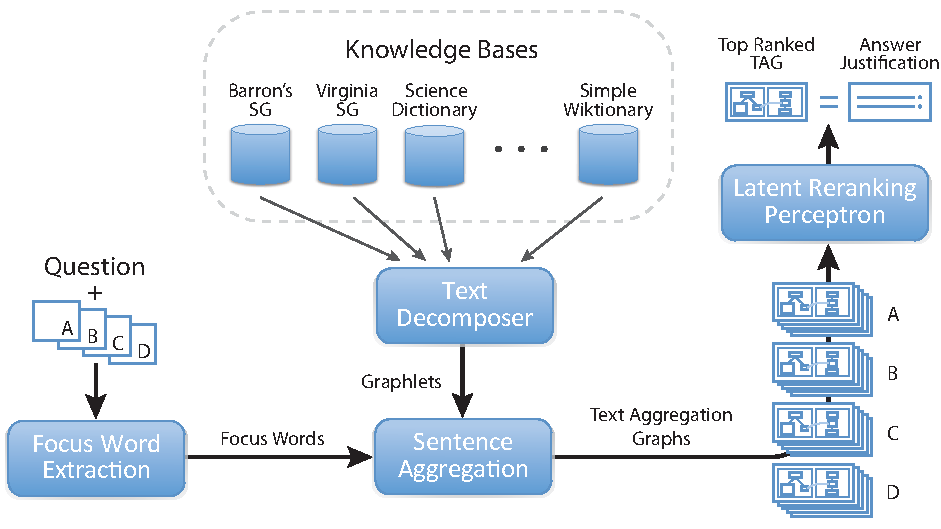
\includegraphics[width=1.0\textwidth]{mainmatter/tacl2015-tig/tag_architecture6c.pdf}

%space{-2mm}
\caption{Our QA approach, which centers on the construction of answer justifications as text aggregation graphs, and ranking them using a model that treats the justification quality as a latent variable.}
%space{-2mm}
\label{fig:architecture}
%\end{center}
\end{figure}

The architecture of our proposed QA approach is illustrated in Figure~\ref{fig:architecture}, and proceeds in a stage-like fashion.  

Prior to the QA task, in an offline process, we decompose sentences from six corpora into a lightly-structured graphical representation (``graphlet'') that splits sentences on clausal and prepositional boundaries (Section~\ref{sec-cl2017:tag}). As shown later, this is fundamental to the creation and evaluation of answer justifications.  All other stages of the framework occur online. 

The QA pipeline receives as input questions with multiple choice answers, similar to the questions shown in Table~\ref{tab:inferenceexamples}, and proceeds as follows. First, the questions are fed into a focus word extractor (Section \ref{sec-cl2017:focuswords}) that produces a weighted list of the keywords from both the question and answer candidates, sorted in descending order of their likely relevance to the information needed in the question. These keywords are used by the sentence aggregation component (Section \ref{sec-cl2017:tag}) to create an exhaustive list of potential answer justifications, for each answer candidate.  These answer justifications are in the form of text aggregation graphs (TAGs), each composed of two to three graphlets produced by the above preprocessing step.

After the sentence aggregation step, each of the multiple choice answers has a long list of candidate justifications.  Because of the large number of candidate justifications created for each question/answer pair (typically tens or hundreds of thousands), we filter the list to include only the top $k$ justifications based on an inexpensive score, implemented as the sum of the weights of the focus words present in each justification\footnote{We keep ties in this filtered list, which, due to the simplicity of the score, may increase the size of the filtered lists considerably. For example, if $k=25$, it is common that the filtered list includes between $100$ and $1,000$ candidate justifications.}. 
Using the focus words, we extract a number of features from each candidate justification that measure how well the justification answers the question (Section ~\ref{sec-cl2017:scoring}), and present this information to a latent-variable perceptron ranker (Section~\ref{sec-cl2017:perceptron}).  This learning framework learns which answer candidate is correct based on the candidate justifications, while also jointly learning to rank justification quality as a latent variable, selectively elevating good answer justifications to the top of the list.  

The candidate answer with the highest-scoring justification is taken to be the correct answer.  While the justification is expressed in the form of a text aggregation graph to make it easier to assemble and evaluate, we use the original sentences from the knowledge base used to construct that text aggregation graph as a human-readable justification for why that answer candidate is correct. 

\section{Focus Word Extraction}
\label{sec-cl2017:focuswords}


%
% Focus word extraction example
%
\begin{table*}[t]
\caption{{Focus word decomposition of an example question, suggesting the question is primarily about measuring the speed of walking, and not about turtles or paths. (Correct answer: ``a stopwatch and meter stick.'') 
For a given word: 
\emph{Conc} refers to the psycholinguistic concreteness score,
\emph{Tag} refers to the focus word category (\emph{FOCUS} signifies a focus word, \emph{EX} an example word, \emph{ATYPE} an answer-type word, and \emph{ST} a stop word),
\emph{Score} refers to the focus word score, and
\emph{Weight} refers to the normalized focus word scores. 
}}
\begin{center}
\begin{footnotesize}
\addtolength{\tabcolsep}{-1.7pt}  
\begin{tabular}{r|cccccccccccc}
Words & What	& tools	& could & determine & the  & {\bf speed} & of   & turtles & {\bf walking} & along & a    & path ? 		\\
Conc  & 2.0A    & 4.6C  & 1.3A  & 2.1A      & 1.4A & {\bf 3.6}   & 1.7A & 5.0C    & {\bf 4.1}     & 2.1A  & 1.5A & 4.4C 		\\
Tag	  & ST      & ATYPE & ST    & ST        & ST   & {\bf FOCUS} & ST   & EX      & {\bf FOCUS}   & ST    & ST   & EX   		\\
Score & --      & 1     & --    & --        & --   & {\bf 14}    & --   & 2       & {\bf 14}      & --    & --   & 3			\\
Weight& --      & 0.03  & --    & --        & --   & {\bf 0.41}  & --   & 0.06    & {\bf 0.41}    & --    & --   & 0.09		\\
\end{tabular}
\addtolength{\tabcolsep}{1.7pt}  
\end{footnotesize}

\label{tab:focusexample}
\end{center}
\end{table*}


Questions often contain text that is not strictly required to arrive at an answer, and that can introduce noise into the answering process. 
This is particularly relevant for science exams, where questions tend to include a narrative or example for the benefit of the reader, and this extra text can make determining a question's \emph{information need} more challenging. 
%
%Elementary science exam questions are often crafted to test a student's knowledge of a single concept, process, or model.
%While some exam questions are short and direct {\em (e.g. What does a thermometer measure?)}, others embed the question in a narrative or example, and we first have to distill what the question is about before we're able to answer.  
For example, the question in Table~\ref{tab:focusexample} could be simplified to {\em What tools can be used to measure speed?}, but instead grounds the question in an example about turtles walking along a path.  As a first step in answering, we need to identify whether the focus of the question is about {\em speed}, {\em turtles}, {\em walking}, or {\em paths}, so that we can appropriately constrain our intersentence aggregation, and decrease the chance of generating noisy or unrelated justifications. 

Note that the {\em focus word} terminology was first introduced in the context of factoid QA, where it represents the question word or phrase that is indicative of the expected answer type, which is then used to constrain the search for candidate answers~\cite{Harabagiu:00,Moldovan:2003:PIE:763693.763694}. For example, {\em capital} is the focus word in the question {\em What is the capital of France?}. This information is used to constrain the search for answers to  entities that are of names of cities. 
In contrast, such words (e.g., {\em tools} for the previous exam question) are often of low importance for multiple choice science exams, as this information is already implicitly provided in the multiple choice answers.  Instead, our task is to identify the central concept the question is testing (e.g., {\em  measuring speed}), and to eliminate words that are part of an example or narrative (e.g., {\em  turtle, path}) that are unlikely to contribute much utility (or, may introduce noise) to the QA process. However, because at a high level focus words identify the information need of a question, which is what we aim to do as well, we continue to use the same terminology in this work.

Our approach borrows from cognitive psychology, which suggests that elementary school students tend to reason largely with concrete concepts (i.e., those that are easy to mentally picture), because their capacity for abstract thinking develops much more slowly into adulthood (e.g., Piaget ~\citeyear{Piaget1954}).  Recently Brysbaert et al. ~\citeyear{brysbaert:2014} collected a large set of psycholinguistic concreteness norms, rating 40 thousand generally known English lemmas on a numerical scale from 1 (highly abstract) to 5 (highly concrete).  We have observed that highly abstract words (e.g., {\em expertise:1.6, compatible:2.3, occurrence:2.6)} tend to be part of a question's narrative or too abstract to form the basis for an elementary science question, while highly concrete words (e.g., {\em  car:4.9, rock:4.9, turtle:5.0)} are often part of examples.  Words that are approximately 50\% to 80\% concrete {\em (e.g., energy:3.1, measure:3.6, electricity:3.9, habitat:3.9)} tend to be at an appropriate level of abstraction for the cognitive abilities of elementary science students, and are often the central concept that a question is testing.\footnote{
While the above concreteness thresholds may be particular to elementary science exams, we hypothesize that the information need of a question tends to be more abstract than the examples grounding that question.  We believe this intuition may be general and applicable to other domains.
}

Making use of this observation, we identify these focus words with the algorithm below. The algorithm is implemented as a sequence of ordered sieves applied in decreasing order of precision~\cite{Lee:13}. Each of the five sieves attempts to assign question words into one of the following categories\footnote{This same process is used to extract focus words for each of the multiple choice answer candidates, though it is generally much simpler given that the answers tend to be short.}: 

\begin{enumerate}

\item {\bf Lists and sequences:} Lists in questions generally contain highly important terms.  We identify comma delimited lists of the form {\small {\tt X, Y, ..., <and/or> Z}} (e.g., {\em sleet, rain, and hail}). Given the prevalence of questions that involve causal or process knowledge, we also identify from/to sequences (e.g., {\em from a solid to a liquid}) using paired {\tt prep\_from} and {\tt prep\_to} Stanford dependencies~\cite{de2008stanford}. 

\item {\bf Focus words:} Content lemmas (nouns, verbs, adjectives, and adverbs) with concreteness scores between 3.0 and 4.2 in the concreteness norm database of Brysbaert et al. ~\citeyear{brysbaert:2014} are flagged as focus words. 

\item {\bf Abstract, concrete, and example words:} Content lemmas with concreteness scores between 1.0 and 3.0 are flagged as highly abstract, while those with concreteness scores between 4.2 and 5.0 are flagged as highly concrete.  Named entities recognized as either durations or locations (e.g., {\em In New York State}) are flagged as belonging to examples.  

\item {\bf Answer type words:} Answer type words are flagged using both four common syntactic patterns shown in Table~\ref{tab:answertypewords}, as well as a short list of transparent nouns (e.g., {\em kind, type, form}). 

\item {\bf Stop words: } A list of general and QA-specific stop words and phrases, as well as any remaining words not captured by earlier seives, are flagged as stop words.

\end{enumerate}

\begin{table*}[t]
\caption{{Syntactic patterns used to detect answer type words.  Square brackets represent optional elements. }}
\begin{center}
\begin{footnotesize}
\begin{tabular}{ll}
\hline
\multicolumn{1}{l}{Pattern} & \multicolumn{1}{l}{Example} 	\\
\hline
(SBARQ (WHNP (WHNP (WDT) {\bf (NN)) [(PP)]}...						& What {\em kind of energy} ...    	\\
(SBARQ (WHNP (WP)) (SQ (VBZ is) {\bf (NP)}...	 					& What is {\em one method} that ... 	\\
(S (NP (NP (DT A) {\bf (NN)}) (SBAR (WHNP (WDT that)) ...			& A {\em tool} that ..					\\
(S (NP {\bf (NP)} (PP)) (VP (VBZ is) ...    						& The {\em main function} of ... is to ...	\\

\end{tabular}
\end{footnotesize}

\label{tab:answertypewords}
\end{center}
\end{table*}





{\flushleft {\bf Scoring and weights:}} We then assign a score to each question word based on its perceived relevance to the question as follows. 
Stop words are not assigned a score, and are not included in further processing.
All answer type words are given a score of 1.  Words flagged as abstract, concrete, or example words are sorted based on their distance from the concreteness boundaries of 3.0 (for abstract words) or 4.2 (for concrete words), where words closer to the concreteness boundary tend to be more relevant to the question, and should receive higher scores.
These words are then given incrementally increasing scores starting at 2 for the most distant word, and increasing by one until all words in this category have been assigned a score.
To create an artificial separation between focus words and the less relevant words, and to encourage our intersentence aggregation method to preferentially make use of focus words, we assign all focus words a uniform score 10 points higher than the highest-scoring abstract, concrete, or example word.  
Finally, list words, the most important category, receive a uniform score one higher than focus words.  The scores of all words are converted into weights by normalizing the scores to sum to one. 
An example of the scoring process is shown in Table~\ref{tab:focusexample}. 

It is important to note that the proposed focus word extraction algorithm is simple and leaves considerable room for improvement. We hypothesize that better algorithms could be implemented by switching to a learning-based approach. However, the simple unsupervised algorithm proposed requires no data annotations, and it captures the crucial intuition that some words in the question  contribute more towards the overall information need than others.  We demonstrate that this has a considerable impact on the performance of our overall QA system in the ablation studies discussed in Section~\ref{sec-cl2017:controls}.





\section{Text Aggregation Graphs}
\label{sec-cl2017:tag}

\begin{figure}[t!]
\begin{center}
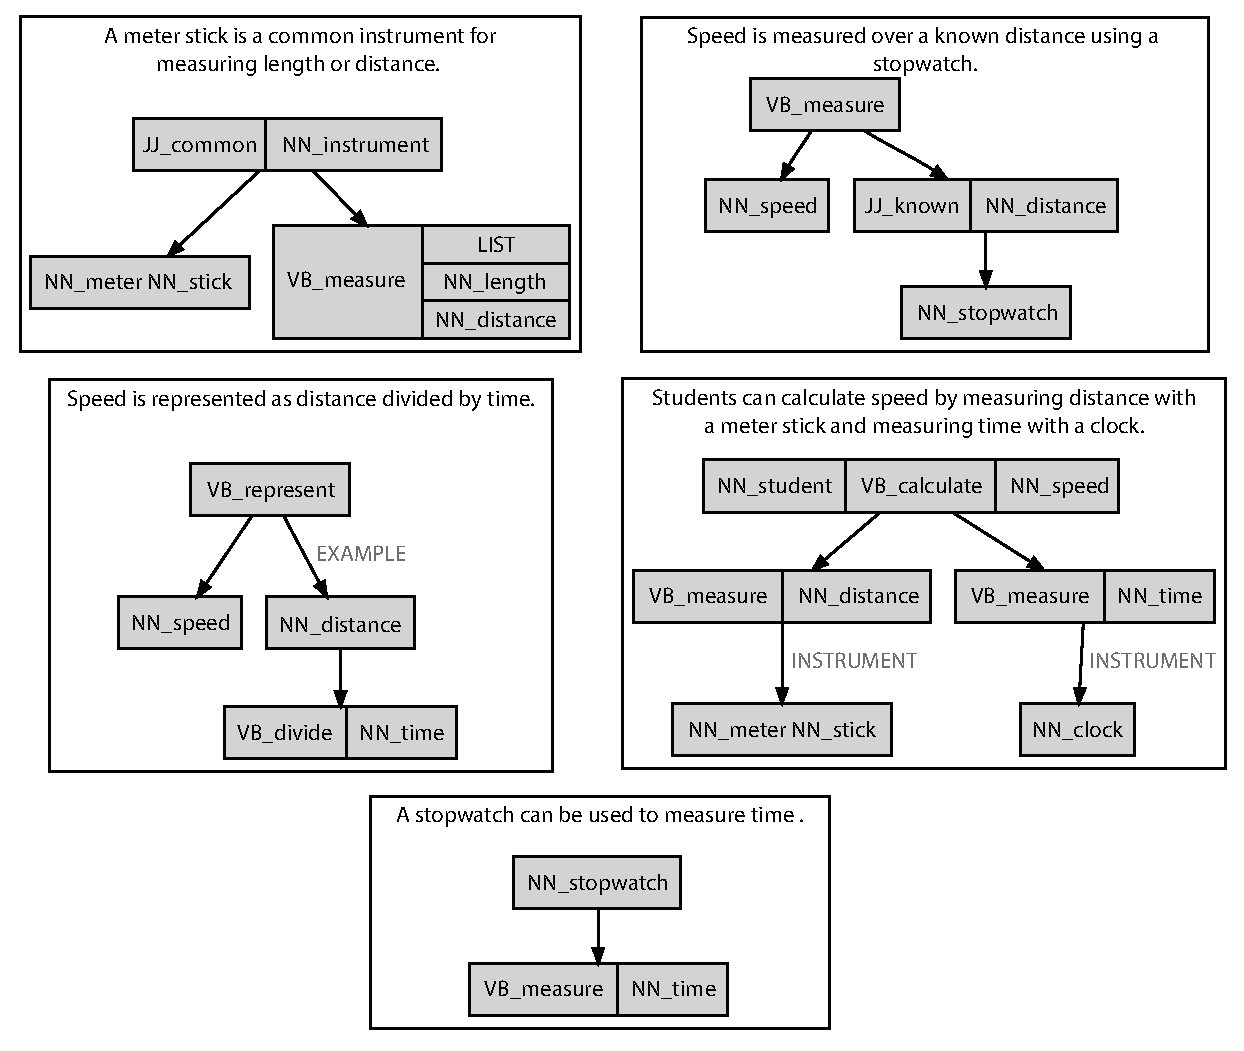
\includegraphics[width=115mm]{mainmatter/tacl2015-tig/example_graphlets1.pdf}
%	\centering
%	\begin{minipage}[b]{0.4\textwidth}	
%		\includegraphics[scale=0.4]{meter_length_distance.pdf}
%	\end{minipage}
%	\hfill
%	\begin{minipage}[b]{0.4\textwidth}	
%		\includegraphics[scale=0.4]{speed_distance_stopwatch.pdf}
%	\end{minipage}
%
%
%	\begin{minipage}[b]{0.4\textwidth}	
%		\includegraphics[scale=0.4]{speed_distance_time.pdf}
%	\end{minipage}
%	\hfill
%	\begin{minipage}[b]{0.4\textwidth}	
%		\includegraphics[scale=0.4]{speed_meter_clock.pdf}
%	\end{minipage}
\end{center}	
%space{-2mm}
\caption{Five example graphlets for five sentences that could be aggregated together in different combinations to justifiably answer the question \emph{What tools could determine the speed of turtles walking along a path? (Answer: stopwatch and meter stick)}.  Each graphlet contains one or more information nuggets (grey boxes) composed of one or more terms.  For example, the graphlet for the sentence \emph{A stopwatch can be used to measure time} contains two information nuggets.  Edges between nuggets within a graphlet are shown with arrows, where a subset of these edges are labelled (e.g., \emph{EXAMPLE, INSTRUMENT}), and the rest are unlabelled. 
}
%space{-5mm}
\label{fig:conceptexamples}
%\end{center}
\end{figure}




Semantic drift, or the tendency for a graph traversal to drift to unrelated topics,
constitutes a major hurdle for lexical semantic QA models.  
This was noted recently by Fried et al.~\citeyear{fried2015higher}, who proposed an approximation of inference for QA as the traversal of a graph that connected concepts (words or lexicalized syntactic dependencies) along lexical semantic associations. While this method is robust and performs better than approaches relying on alignment or embedding models alone, it does not have a good way of keeping an inference on-context when traversing the concept association graph.
Moreover, even when a correct answer is selected, these methods operate on sets of probabilities over word distributions, and are unable to provide a compelling human-readable explanation to the user as to why a given answer is correct. 

To address these issues, we propose to construct multi-sentence answer justifications using a  sentence aggregation method that combines the robustness of word-level connections with sentence-level context.  
Our approach works in two steps, both of which are performed offline, i.e., before the actual QA process. First, we decompose sentences that are likely to justify science exam answers (e.g., from knowledge bases such as study guides) into smaller units based on clausal and prepositional phrase boundaries. Intuitively, this allows us to maintain sufficient context to control semantic drift, while, at the same time, mitigating the sparsity of complete sentences.  
Following previous QA terminology, we call these smaller units,  which represent clauses or prepositional phrases, {\bf information nuggets}~\cite{Voorhees:2003}. We connect two information nuggets within the same sentence if there are any syntactic dependencies that connect any words in these nuggets. We call the resulting graph of these information nuggets, which represents an entire sentence, a \textbf{graphlet}. 
Figure \ref{fig:conceptexamples} shows a number of example graphlets. 
Formally, we transform sentences into graphlets using the following algorithm:


\begin{enumerate}

\item{\textbf{Parse knowledge base sentences: } 
All knowledge base sentences are syntactically parsed using the Stanford CoreNLP toolkit~\cite{manning2014stanford}.}

% ms: let's use {\tt } for syntactic dependencies, and {\em } font for text.

\item {\textbf{Decompose sentences into information nuggets: \label{step:creatinggraphlets}} 
For each sentence, beginning at the root of the dependency graph, we traverse the dependency graph and segment the sentence into nuggets along clausal complements ({\tt ccomp, xcomp}), adverbial and relative clause modifiers ({\tt advcl, rcmod}), reduced non-finite verbal modifiers ({\tt vmod}), and a subset of empirically determined prepositional phrases.\footnote{The full list of prepositional dependencies along which we split is: {\tt prep\_with, prep\_through, prep\_from, prep\_to, prep\_as, prep\_into, prep\_by, prep\_in, prep\_such\_as, prep\_because\_of, prep\_over, prep\_on, prep\_between, prepc\_as, prepc\_by, prepc\_of, prepc\_with, prepc\_after, prepc\_for, prepc\_before, prep\_before, prep\_after, prep\_during, prepc\_during, prepc\_because\_of, prep\_without,} and {\tt prepc\_without}.}
}

\item {\textbf{Segment nuggets into terms: }
Each nugget is segmented into one or more terms.  A term is nominally a single word, but we join both noun compounds and lists into single terms.  Noun compounds (e.g., \emph{meter stick} in Figure \ref{fig:conceptexamples}) are detected using the {\tt nn} dependency tag, and lists of words (e.g., \emph{sleet, rain, hail, or snow}) are detected through the same patterns used by the focus word extractor (see Section \ref{sec-cl2017:focuswords}).
}


\item {\textbf{Construct graphlets:} Two nuggets within a graphlet are connected if any of the words in one nugget have links in the syntactic dependency tree with words in the other nugget. } 

\item {\textbf{Label a subset of the graphlet  edges:} In general, to increase robustness, edges between nuggets are unlabelled.  The exceptions to this are a small set of high-confidence labels: the label {\tt definition} derived from the semi-structured dictionary resources which distinguish between a defined word and its definition, and the labels {\tt instrument, process, example, temporal}, and {\tt contrast} derived from prepositional dependencies.\footnote{More specifically, in our method the {\tt instrument} label corresponds to the dependencies {\tt prep\_with, prep\_through}, and {\tt prep\_by}.  The label {\tt process} corresponds to the dependencies {\tt prep\_from, prep\_to, prep\_into, prep\_because\_of}, and {\tt prepc\_because\_of}.  The {\tt example} label corresponds to {\tt prep\_as, prepc\_as, prep\_such\_as}, and {\tt prepc\_such\_as}.  The {\tt temporal} label corresponds to {\tt prep\_before, prepc\_before, prep\_after, prepc\_after, prep\_during} and {\tt prepc\_during}.  Finally, the {\tt contrast} label corresponds to {\tt prep\_without} and {\tt prepc\_without}.}}

\item {\textbf{Remove stop-words:}  Finally, we remove any stop words, as well as words that are not nouns, verbs, or adjectives.  Any nuggets that are empty after this filtering are removed. }

\end{enumerate}

\begin{figure}[t!]
\begin{center}

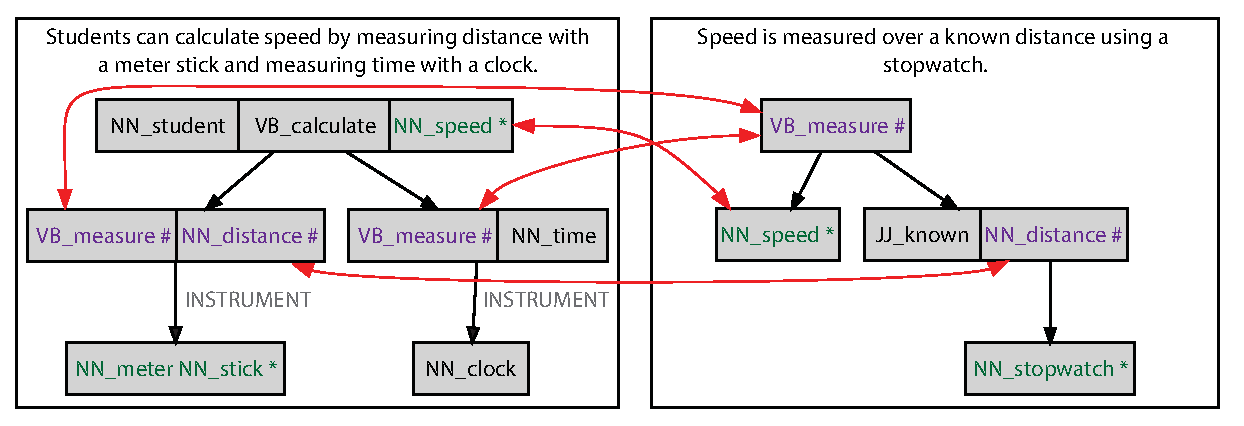
\includegraphics[width=115mm]{mainmatter/tacl2015-tig/tag_connection_example2.pdf}
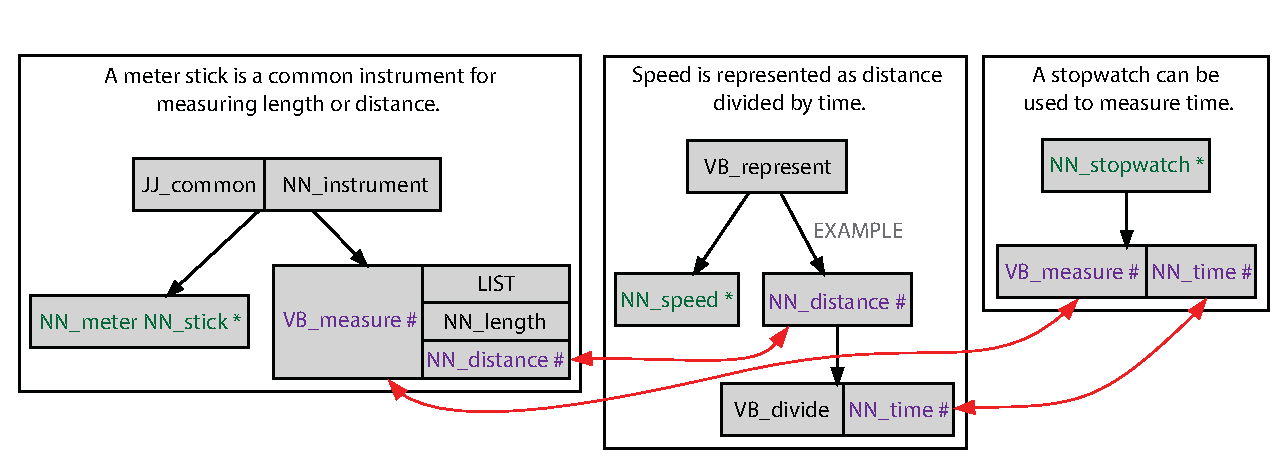
\includegraphics[width=115mm]{mainmatter/tacl2015-tig/tag_example2.pdf}

%space{-2mm}
\caption{
Two example Text Aggregation Graphs (TAGs) that justifiably answer the question \emph{What tools could determine the speed of turtles walking along a path} for the answer \emph{a stopwatch and meter stick}. Asterisks (*) denote that a given term is either a question or answer focus word, while pounds (\#) denote terms that are not found in the question or answer, but which are shared between graphlets.  Links between the graphlets in a given TAG are highlighted. (top) A two-sentence TAG, where the edges between graphlets connect on a focus word \emph{(speed)} and other words shared between the graphlets \emph{(distance, measure)}. (bottom) A three-sentence TAG, where the edges between graphlets connect entirely on shared words between the graphlets \emph{(distance, measure, time)} that are not focus words.
}
%space{-5mm}
\label{fig:tag_example}
\end{center}
\end{figure}


After the sentences have been transformed into graphlets, we construct candidates for multi-sentence justifications by connecting sentences with any lexical overlap between information nuggets.  We currently connect up to three graphlets into constructs we call \textbf{text aggregation graphs (TAGs)}, where each TAG corresponds to one potential answer justification. 
Figure~\ref{fig:tag_example} shows an example of two TAGs. 
Note that a TAG contains multiple levels of structure: (a) clause-level structure within nuggets, (b) sentence-level structure within graphlets, and (c) intersentence structure within TAGs\footnote{Currently, the graphlets and TAGs make use of lexical and syntactic structure only.  While this provides a robust representation of much of the structure in text, in a future system we would also like to explore adding semantic role and discourse information in our graphlets. Both of these have been shown to be useful, albeit for simpler QA tasks~\cite{Surdeanu:11,jansen14}.}.  
We will exploit this information in the next section, where we design features to capture the fitness of a TAG as a justification for a given answer.



\section{Text Aggregation Graph Features}
\label{sec-cl2017:scoring}

Once candidate answer justifications have been reframed as text aggregation graphs, the TAGs for each answer candidate need to be ranked such that a good justification for the correct answer will be ranked above all other answer justifications for incorrect answers. We describe the features that we extract from TAGs for this ranking in this section, and the latent ranking algorithm in Section~\ref{sec-cl2017:perceptron}.




\begin{table}[]
\caption{{  Features used to score candidate answer justifications represented as TAGs. }} 
\footnotesize{
\begin{tabular}{p{30mm}p{95mm}}
\hline
Feature & Description \\
\hline
\multicolumn{2}{l}{\emph{TAG-level features:}} \\
%numFocus			&	Number of unique Q and A focus words present in the TAG					\\
numFocusQ			&	Number of unique Q focus words present in the TAG						\\
numFocusA			&	Number of unique A focus words present in the TAG						\\
massFocusQ			&	Sum of the unique Q focus word weights present in the TAG				\\
massFocusA			&	Sum of the unique A focus word weights present in the TAG				\\
%\\
%\multicolumn{2}{l}{\emph{Other TAG-level Scores:}} \\
numRepeatedFocus	&	Number of focus words contained in more than one graphlet, with repetition \\
numOtherAnswerF		&	Negative predictor: the number of focus words from other multiple choice answers included in the current TAG.	\\
minConcShared		&	The minimum psycholinguistic concreteness score (i.e., abstractness) of any shared word in the TAG \\
\\
\multicolumn{2}{l}{\emph{Nugget-level features: }} \\
numNugF				&	Number of nuggets that are entirely focus words. \\
numNugFS 			&	Number of nuggets that contain only focus words and shared words. \\
numNugFSO			&	Number of nuggets that contain focus, shared, and other unmatched words. \\
numNugFO			&	Number of nuggets that contain only focus words and other words. \\
numNugS				&	Number of nuggets that contain only shared words. \\
numNugSO			&	Number of nuggets that contain only shared words and other words. \\
numNugO				&	Number of nuggets that contain only other words. \\
% \\
% \multicolumn{2}{l}{\emph{Other Nugget-level features: }} \\
numDefinedFocus		&	Number of nuggets containing only focus words with outgoing {\tt definition} edge \\
numDefinedShared	&	Number of nuggets containing only shared words with outgoing {\tt definition} edge \\
numQLinksFocus		&	Number of nuggets containing only focus words that have an incoming labeled link (e.g., {\tt definition, instrument, process, temporal})  \\
numQLinksShared		&	Number of nuggets containing only shared words that have an incoming labeled link  \\
numNuggetMultiF		&	Number of nuggets that contain more than one focus word\\
\\
\multicolumn{2}{l}{\emph{Bridge features:}} \\
massMaxBridgeScore		&	Bridge graphlets are graphlets that contain at at least one focus word from both the  \\
massMinBridgeScore		&	question and answer, signifying that they are highly relevant to the question and the \\
massDeltaBridgeScore	&	corresponding answer. A   graphlet's bridge score is the sum of this focus word mass.  We calculate the minimum, maximum, and delta (max $-$ min) bridge scores across all graphlets within a TAG. \\
\\



\hline
\end{tabular}
}
\label{tab:features}
\end{table}


\subsection {Features} 
\label{sec-cl2017:featuresandscoring}

We developed a set of TAG features that capture both the type of connections between the graphlets in a TAG, and how well the TAG as a whole relates to the corresponding question--answer pair.
The features can be broadly grouped into count features and mass features. Count features count the integer number of instances of a given event in a TAG -- for example, the number of nuggets that are entirely focus words.  Mass features sum the weights of focus words (as computed in Section~\ref{sec-cl2017:focuswords}) -- for example, summing the weight of all question or answer focus words found either within a single graphlet, or across the entire TAG.

A full list of the features and their descriptions can be found in Table \ref{tab:features}.
%
The features are grouped into three categories: TAG-level, nugget-level, and bridge features. 
The TAG-level features use focus words to evaluate the likelihood that an entire justification is relevant to the question and answer candidate. 
Nugget-level features provide a finer-grained measure of how well the individual sentences in a justification relate to each other by quantifying both \emph{how fully} they are connected (e.g., are all the words in a nugget matched with words in other nuggets, or only some), and what type of words they connect on (e.g., \emph{focus words}, or \emph{other words} not found in the question but shared between sentences).
Separate features encode whether a nugget is all focus words, all shared words, all unmatched words, or any partial combination of these three categories.
Finally, we define a graphlet that contains both question and answer focus words as a \emph{bridge graphlet}, in that its content tends to span or \emph{bridges} the question and answer, and include a set of bridge features for evaluating this subset of highly-relevant graphlets. 




%- TAG = path = answer justification
\begin{figure}[t!]
\begin{center}
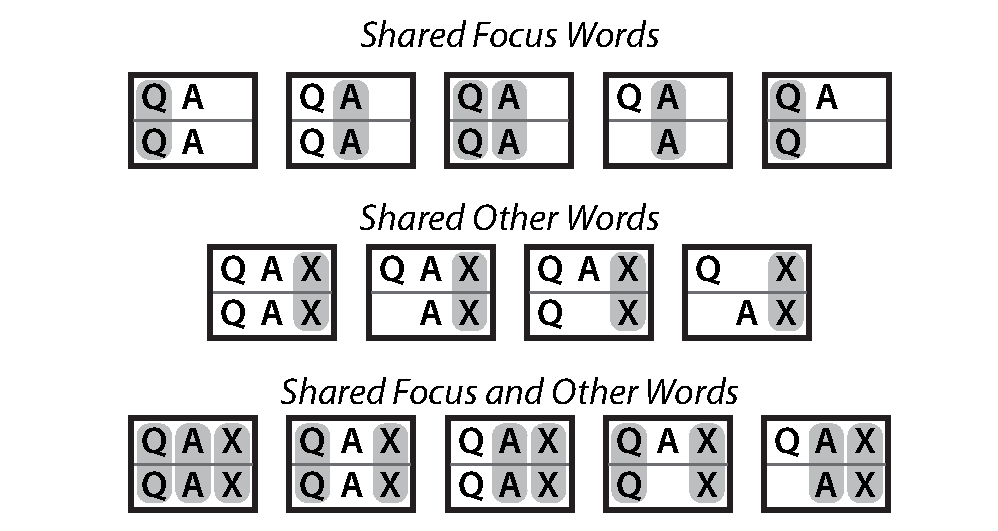
\includegraphics[width=75mm]{mainmatter/tacl2015-tig/connection_types.pdf}
%space{-2mm}
\caption{{Connections between sentences are characterized based on lexical overlap between graphlets.
Here, each box represents a two-sentence TAG, with graphlets stacked vertically.  The presence of question or answer focus words is marked with \emph{Q} or \emph{A}, while the presence of other non-focus words shared between the two graphlets is marked with \emph{X}.  Lexical overlap within a category is highlighted.
}}
%space{-5mm}
\label{fig:connectiontypes}
\end{center}
\end{figure}


\subsection {Modeling Different TAG Types Using Domain Adaptation} % Characterizing Lexical Overlap Between Sentences}
\label{sec-cl2017:characterizing}

Good justifications for an answer may take a variety of forms, from those with little lexical overlap due to the ``lexical chasm''~\cite{Berger:00} between question and answer, to those with a great deal of overlap. For example, of the two TAGs shown in Figure~\ref{fig:tag_example}, in the first TAG both sentences connect on question focus words, while in the second TAG the graphlets only connect on other non-focus words. 

Understanding the connections between sentences in a TAG serves as a robust proxy to modeling discourse structures (e.g., whether the second sentence elaborates on the concepts introduced in the first), which has been previously shown to increase both open-domain and science-domain QA performance~\cite{jansen14}.
This is important in the context of feature representations, because we conjecture that some features may be important across all the ways a justification can connect (so these features should be jointly modelled across connection types), whereas others are specific to certain connection types (so they should be modeled separately by type). As shown in Section~\ref{sec-cl2017:experiments}, this hypothesis is strongly empirically supported.

To model this phenomenon, we adapt a technique from the field of domain adaptation~\cite{daume2007}.
First, we label each of the sentences within a TAG based on whether they contain question focus words and/or answer focus words.  We then characterize the entire TAG by determining whether the words shared between sentences are question focus words, answer focus words, or other non-focus words.  This leads to 14 possible connection types, depicted in Figure \ref{fig:connectiontypes}.\footnote{In practice, for a configuration that allows TAGs of 1 or 2 sentences, we have 15 connection types, including the 14 two-sentence connection types, plus a single-sentence type. We ignore the single-sentence type in this discussion for simplicity, though it is included in our model.}
Second, following Daum{\'e}'s method, we generate 15 versions for each of the features introduced in Section~\ref{sec-cl2017:featuresandscoring}: a generic one that is type independent, and 14 that are affixed by each of the connection types. For example, for a given feature such as \emph{numFocusQ}, we create 15 copies: \emph{numFocusQ, numFocusQ$_1$ ... numFocusQ$_{14}$}, where the subscript (when present) indicates a specific connection type. For a TAG of connection type \emph{i}, only values for the type-specific feature \emph{numFocusQ$_i$} as well as the general feature \emph{numFocusQ} are populated -- all other \emph{numFocusQ$_j$} features are set to a value of zero. This allows the learning algorithm in the next section to learn whether each feature generalizes across connection types, or not. As shown in~\cite{finkel2010hierarchical}, this approach is equivalent to a joint model with a hierarchical prior. 



While the features introduced in Table~\ref{tab:features} apply to justifications containing any number of sentences, characterizing justifications that are longer than two sentences is not straightforward, as the number of connection types (Figure~\ref{fig:connectiontypes}) would become prohibitively large.   We handle three-sentence justifications by treating each as a set of three two-sentence TAGs, and characterize each two-sentence connection individually.  In the case where two groups of sentences have the same connection type, we take the highest scoring version of each overlapping feature.  While this method would extend to justifications of arbitrary length,  justifications longer than three sentences are not currently generated by our system. 



\section{Learning Model}
\label{sec-cl2017:perceptron}

We perform answer selection by focusing on ranking answer {\em justifications} rather then actual answers. 
Our algorithm (detailed in Algorithm \ref{alg:perceptron}) determines the best answer to a given question by first finding the highest-scoring TAG (i.e., justification) out of all the TAGs for each of its candidate answers, and then selecting the corresponding answer candidate.  
This introduces an additional complication during training: while we know which answer candidate is correct, the actual quality of any given TAG is hidden. That is, many TAGs which connect a correct answer to the question do so in the wrong context, producing a poor justification. Conversely, even an incorrect answer can be connected back to the question, otherwise the multiple choice test itself would be too easy. 

We address this issue with a reranking perceptron~\citep{Shen:Joshi:2005,Surdeanu:11} extended with a latent layer that models the correctness of the justifications. 
During training, we take advantage of the assumption that, with enough knowledge coverage, the best TAG for a correct answer will be better than the best TAG for an incorrect one.  As a result, our algorithm optimizes two goals jointly: choosing a good answer for a given question, and justifying it with a human-readable TAG that connects sentences from our knowledge bases.

\subsection {Learning Algorithm}
\label{sec-cl2017:model}

The input to the reranking algorithm consists of a corpus of $n$ training questions, $\boldsymbol{\mathcal{Q}}$, where each $q_i \in \boldsymbol{\mathcal{Q}}$ has a set of $m$ candidate answers, $\boldsymbol{A}$ (in the particular case of the multiple choice test, these are the four multiple choice answers).  Each $a_j \in \boldsymbol{A}$ for a given $q_i$ has a set of TAGs, $\boldsymbol{X_{i,j}}$, which connect $q_i$ to $a_j$.  
Crucially, for a correct answer, we assume that there is {\em at least one} valid TAG $x_c \in \boldsymbol{X_{i,j}}$, which justifies the correctness of the chosen answer. This assumption is similar to the one made by \citet{hoffmann2011knowledge}, who assumed that, for a binary relation extraction task, for each training relation between two entities, $e_1$ and $e_2$, there exists at least one correct sentence that supports the extraction of the given relation among the sentences that contain both $e_1$ and $e_2$.

The learning algorithm is formalized in Algorithm~\ref{alg:perceptron}. The two fundamental building blocks of the algorithm are the functions $P$ and $F$. 
Intuitively, the function $P$ identifies which justifications (or TAGs) for a given answer best explain the answer according to the current model. For example, for the question {\em Which organism is a producer?} and the answer {\em grass}, a good justification selected by function $P$ is a TAG that connects the two sentences: {\em Producer is an organism that produces its own food and is food for other organisms: usually a green plant.} and {\em Grass is a green, leafy plant that often covers the ground.} 
Because $P$ implements a latent operation (i.e., which justification is correct?), its goodness evolves together with the learned model. 
Note that, at this stage, we do not control how many justifications are produced by function P for a given answer other than constraining it to select {\em at least one}. The function $F$ computes the overall score of a given answer by simply averaging the scores of the justifications chosen by $P$. 

More formally, for a given question $q_i$ and candidate answer $a_j$, $P$ chooses a subset of TAGs from $\boldsymbol{X_{i,j}}$ that are deemed correct, according to the current model. $F$ averages the scores of these TAGs to compute the overall score of the answer $a_j$:

\begin{equation}
\label{eq:F}
F(q_i, a_j) = \frac{\sum_{x \in P(q_i, a_j)} \boldsymbol{\Theta} \cdot \Phi(x)}{|P(q_i, a_j)|}
\end{equation}
where the score of a given TAG, $x$, is computed as the dot product between the model's weight vector $\boldsymbol{\Theta}$  and the individual TAG's feature vector $\Phi(x)$. 

Given the functions $P$ and $F$ that control the latent operation of choosing valid answer justifications, the algorithm proceeds similarly to the reranking perceptron~\citep{Shen:Joshi:2005}. If a prediction, i.e., a choice for the correct answer for a given question (line 6), is incorrect (line 7), the algorithm updates its parameter vector, $\boldsymbol{\Theta}$, by adding all valid justifications of the correct answer as produced by $P$ (line 9), and subtracting all TAGs considered valid for the current top answer (line 12). 


The fundamental operation here is thus the implementation of $P$. For their classification task, Hoffman et al. implement this function as an edge-cover\footnote{
\rev{The edge-cover of a graph is a subset of the graph's edges such that each node in the graph is connected to at least one edge in the subset.  For the task of relation extraction, \citet{hoffmann2011knowledge} construct a fully-connected graph with nodes for each supporting sentence from the corpus and nodes for each relation.  Their approach to relation extraction learns which relations to extract from the supporting sentences by finding the \textit{best} edge-cover for the graph.}} problem, which guarantees that the overall score for the correct label (similar to our $F$ function) is maximized and at least one sentence supports the correct classification.  
For our reranking task, we found that a conservative interpretation of this, where {\em exactly} one justification is chosen, performed the best.\footnote{In fact, we found that performance consistently dropped as the number of justifications chosen by $P$ increased.} That is, $P$ returns only the top TAG with the highest score according to the dot product with the current $\boldsymbol{\Theta}$. 
We discuss the other extreme, i.e., using all TAGs, in Section \ref{sec-cl2017:controls} (when taken to this level, the latent layer is essentially disregarded entirely, assuming that each TAG for a correct answer is correct, and that each TAG for an incorrect answer is incorrect).  As discussed there, this performed far worse.


%\begin{algorithm}[t]
%%\SetAlgoLined
%%\linesnumbered
%\LinesNumbered
%\KwIn{  $ $\\
%$T$ -- the number of training epochs\;
%$\boldsymbol{\Sigma}$ -- the set of $n$ training questions, each of which has $m$ answer candidates\;
%$\boldsymbol{X_{i,j}}$ -- the set of all paths connecting a question $q_i$ with a candidate answer $a_j$\;}
%\KwOut{ \\
%$\boldsymbol{\Theta}$ -- parameter vector\;}
%\Begin{
%% {\small \tcp{Initialize parameter vector}}
%$\boldsymbol{\Theta} = \boldsymbol{0}$\;
%\For{$t\leftarrow 1$ \KwTo $T$}{
%	\For{$i\leftarrow 1$ \KwTo $n$} {
%			$k = \argmax_{j = 1, \dots, m} F(q_i, a_j)$\; 
%			\If{$k \ne 1$}{
%				\For{$x \leftarrow P(q_i, a_1)$}{
%					$\boldsymbol{\Theta} = \boldsymbol{\Theta} + \Phi(x)$\;
%				}
%				\For{$x \leftarrow P(q_i, a_k)$}{
%					$\boldsymbol{\Theta} = \boldsymbol{\Theta} - \Phi(x)$\;
%				}
%			}
%%			compute $ y_1 = F(a_1, X_1)$\\
%%			\For{$j\leftarrow 2$ \KwTo $m$} {
%%				%$z_{j}^{*}$ = $ argmax_{\bar{z_{j}}}$($\theta \cdot \bar{z_{j}}$)\; 
%%				compute $ y_j = F(a_j, X_j)  $\; 
%%				}
%%		find $p = argmax_m(Y) $\\
%%		\If{$ (y_1 - y_{p}) < \lambda $}{
%%			$ \bar{\theta} = \bar{\theta} + (\Phi(X_1) - \Phi(X_{p})) \tau $ \;
%%		}
%}
%}
%}
%\Return{$\boldsymbol{\Theta}$}
%\vspace{5mm}
%\caption{{\footnotesize Learning algorithm for the latent reranking perceptron. We consider, without loss of generality, that the correct answer appears at position 1 in training.}}
%\label{alg:perceptron}
%\end{algorithm}
\begin{algorithm}[t]                      % enter the algorithm environment
                 % and a label for \ref{} commands later in the document
\begin{singlespace}
                 \small
\begin{algorithmic}[1]                    % enter the algorithmic environment
    \STATE \textbf{Input:}{$ $\\
$T$ -- the number of training epochs}\\
$\boldsymbol{\mathcal{Q}}$ -- the set of $n$ training questions, each of which has $m$ answer candidates\\
$\boldsymbol{X_{i,j}}$ -- the set of all TAGs connecting a question $q_i$ with a candidate answer $a_j$\\
    \STATE \textbf{Output:}{ $\boldsymbol{\Theta}$ -- parameter vector\\}
    \STATE $\boldsymbol{\Theta} = \boldsymbol{0}$\;
	\FOR{$t\leftarrow 1$ --to-- $T$}
		\FOR{$i\leftarrow 1$ --to-- $n$} 
			\STATE $k = \argmax_{j = 1, \dots, m} F(q_i, a_j)$
			\IF{$k \ne 1$}
				\FOR{$x \leftarrow P(q_i, a_1)$}
					\STATE $\boldsymbol{\Theta} = \boldsymbol{\Theta} + \Phi(x)$
				\ENDFOR
				\FOR{$x \leftarrow P(q_i, a_k)$}
					\STATE $\boldsymbol{\Theta} = \boldsymbol{\Theta} - \Phi(x)$
				\ENDFOR
			\ENDIF
		\ENDFOR
	\ENDFOR
	\RETURN $\boldsymbol{\Theta}$
\end{algorithmic}
\end{singlespace}
\caption{ Learning algorithm for the latent reranking perceptron. We consider, without loss of generality, that the correct answer appears at position 1 in training.}   
\label{alg:perceptron}
\end{algorithm}



{\flushleft{\bf Inference:}}
%\paragraph{Inference}
During inference, the algorithm ranks all candidate answers for a given question in descending order of their score (as given by $F$, but using the averaged parameter vector, $\boldsymbol{\Theta_{avg}}$) and returns the top answer.

{\flushleft{\bf Practical concerns:}}
Two practical issues were omitted in Algorithm~\ref{alg:perceptron} for clarity, but improved performance in practice. First, we used the averaged percetron at inference time~\citep{Collins:2002:DTM}. That is, instead of using the latest $\boldsymbol{\Theta}$ after training, we averaged all parameter vectors produced during training, and used the averaged vector, $\boldsymbol{\Theta_{avg}}$, for inference.

Second, we used a large-margin perceptron, similar to~\citet{Surdeanu:11}. In particular, we update the model not only when the predicted answer is incorrect (line 5), but also when the current model is not confident {\em enough} -- that is, when the predicted answer is correct, but the difference in $F$ scores between this answer and the second predicted answer is smaller than a small positive hyper parameter $\tau$. 




\section{Experiments}
\label{sec-cl2017:experiments}

\subsection{Data}
\label{sec-cl2017:data}


{\flushleft {\bf Questions:}} We assembled a corpus of 1,000 third to fifth grade standardized elementary school science exam questions, consisting of 346 publicly available questions gathered from standardized exams in 12 states, as well as 654 additional questions from an exam generating service that are not publicly available. 
All questions are multiple choice with four possible answer candidates. Questions vary in length from 1 to 6 sentences, while the four multiple choice answer candidates are generally either single words or short phrases. 
Because of the small size of this corpus, our models were evaluated using 5-fold crossvalidation, with 3 folds for training, one for development, and one for test. 

{\flushleft {\bf Knowledge bases:}} Sentences from six text resources served as input for TAG generation.  Five of these resources are in the science domain and include two state-specific science exam study guides, a teacher's manual, a children's science dictionary, and a set of exam review flashcards.  Each of these in-domain resources was selected to be at a third-to-fifth grade knowledge level, and contained between 283 and 1,314 sentences (for a total of 3,832 in-domain sentences).  
The Simple Wiktionary\footnote{\url{http://simple.wiktionary.org}} was included as a large open-domain dictionary resource written at knowledge level similar to that of the exam questions.  Starting with over 24,000 definitions, we filtered these to include only definitions for nouns, verbs, and adjectives, for a total of 17,473 sentences after filtering.

\subsection{Tuning}
\label{sec-cl2017:tuning}
We tuned the following hyperparameters once on the development data to optimize both performance and stability.

{\flushleft \textbf{Number of candidate justifications:}} 
Each of the multiple choice answers can have a large number of candidate justifications.  To reduce runtime and assist learning, we filter this initial list of TAGs to include only a subset of TAGs with a high focus word mass. We kept all justifications tied for focus mass with the justification in 25th place, resulting in a variable number of TAGs for each QA pair.  For our dataset, the mean number of TAGs for each QA pair was 141. \\

{\flushleft \textbf{Perceptron Hyperparameters:}} We investigated the perceptron hyperparameters using a coarse grid search\footnote{For each hyperparameter, we systematically tried values differing by an order of magnitude (rather than by small increments) to find our final settings.} and found a stable optimum with 10 epochs, a $\tau$ of 1.0, burn in of 5 epochs (i.e., the weight updates were not added to the average weights for the first five epochs), and a learning rate (which dampened the updates to the weight vector) of 0.1. Since model results can vary depending on the random seed used for initialization, rather than using a single perceptron we use an ensemble of 50 perceptron models initialized with random weights.  These models are combined in a by voting -- each model casts a single vote for an answer candidate to each question (distributing the vote only in the case of ties), then the answer candidate with the most votes is selected.\\

{\flushleft \textbf{Feature Normalization:}} To minimize the effect of outliers in the feature space, we log-transformed the feature values, and then rescaled each feature independently to lie within the range of $-1$ to $1$, using the formula
\mbox{$normalized  = lower + (original - min)\frac{(upper - lower)}{(max - min)}$},
where $upper$ and $lower$ are the desired boundaries for the normalization ($1$ and $-1$, respectively), $max$ and $min$ are the maximum and minimum values for the corresponding feature across the training dataset, and $normalized$ is the result of normalizing $original$.
Note that during testing it is possible to see feature values outside of their known $[min, max]$ interval, which means that after normalization their values will fall outside the $[-1, 1]$ interval. We do not do any additional post-processing for these values.


\subsection{Baselines}
\label{sec-cl2017:baselines}

We include the following baselines: 

{\flushleft {\bf Random:}} selects an answer randomly.
{\flushleft {\bf Information retrieval (IR):}} ranks answers using an approach similar to the baseline model in \citet{jansen14}, which uses features that measure cosine similarity over {\em tf-idf} vectors \citep[][Ch. 6]{manning08} to rank answer candidates in a ``learning to rank'' (L2R) framework (see also Section \ref{sec-naacl2015:models}).  
Traditionally, with retrieval systems, short answers to questions are dynamically constructed from larger parent documents, and the top-scoring answer (defined as the answer with the highest {\em tf-idf} score between that answer candidate and a query vector made from the question) is taken to be the winner.  Here we adapt this setup to multiple choice exams by: (a) using query vectors that contain words from both the question and multiple choice answer candidate, and (b) generating features from the top {\em tf-idf} score for each answer candidate in a given question, which are then combined in the learning-to-rank framework.  We then take the short passage retrieved by the system as a justification for why that answer candidate is correct. 

Documents are constructed across the six knowledge bases by dividing each corpus by subsection (for texts), by definition (for dictionaries), or by flashcard.  We implemented the document indexing and retrieval system using Lucene\footnote{\url{http://lucene.apache.org}}.  Each sliding window of $N$ sentences in a given document served as a potential answer justification. Using the development questions, we empirically determined that a two-sentence window performed best, though performance did not significantly differ for window sizes between one and five sentences.  This  model generates two features: a cosine similarity score between the query vector and the best-scoring candidate answer justification in a given corpus, and a linear model that combines this cosine similarity with the cosine similarity between the query vector and the entire document, blending both local (answer justification) and global (document) context. 

Because our six corpora are of different genres (study guide, teachers guide, dictionary, flashcards), domains (science-domain vs. open-domain), and lengths (300 to 17,000 sentences), we implement six separate {\em tf-idf} models, each containing documents only from a single corpus. We then combine the two retrieval features from each model (12 features total) into a ranking perceptron \citep{Shen:Joshi:2005,Surdeanu:11} to learn which knowledge bases are most useful for this task.  This ensemble retrieval model produces a single score for each multiple choice answer candidate, where the top-scoring answer candidate is selected as the winner.  The top-scoring answer justifications from each of the six retrieval models then serve as justifications. 


 
{\flushleft {\bf Jansen et al. (2014):}} the best-performing combined lexical semantic and IR model of \citet{jansen14}, which was shown to perform well for open domain questions.  Similar to the IR model, we adapted this model to our task by including six separate lexical semantics (i.e. word embedding) language models \citep{mikolov13,mikolov10}, each trained on one of the six knowledge bases.  Two features that measure the overall and pairwise cosine similarity between a question vector and multiple choice answer candidate vector are included.  The overall similarity is taken to be the cosine similarity of the composite vectors of both the question and answer candidate, obtained by summing the vectors for the individual words within either the question or answer candidate vectors, then renormalizing these composite vectors to unit length.  The pairwise similarity is computed as the average pairwise cosine similarity between each word in the question and answer candidate.  Two features from each of the six lexical semantics models are then combined with the two features from each of the IR models (24 features total) as above using a ranking perceptron, with the top-scoring answer candidate taken as correct.  Because the lexical semantics features do not easily lend themselves to constructing answer justifications, no additional human-readable justifications were provided by this model. 


\subsection{Results}
\label{sec-cl2017:results}

Here we first investigate the performance of two variants of the TAG model with respect to justification length.  We then compare the best-performing model with the baselines, and show that the TAG and IR models can be combined to increase performance. We use the standard implementation for precision at 1 \citep[P@1;][]{manning08} and a tie-aware implementation of mean reciprocal rank \citep[MRR;][]{mcsherry2008}.  All statistical significance tests were performed using one-tailed bootstrap resampling with 10,000 iterations (see Section \ref{sec-naacl2015:results}, Footnote \ref{footnote:bootstrap} for implementation).



%
% Performance versus path length
%
\begin{table}[t]
\small
\begin{center}
%\begin{tabular}{p{0.3mm}p{55mm}llll}
\begin{tabular}{lllll}
\multicolumn{1}{l}{ } & \multicolumn{1}{l}{ } & \multicolumn{1}{l}{P@1} & \multicolumn{1}{l}{ } & \multicolumn{1}{l}{MRR} \\
\multicolumn{1}{l}{ Model } & \multicolumn{1}{l}{P@1} & \multicolumn{1}{l}{Impr.} & \multicolumn{1}{l}{MRR} & \multicolumn{1}{l}{Impr.} \\
\hline
\multicolumn{5}{l}{Normal}\\
\hline
1G					& 35.33			& --				& 59.26  		&	--  \\
2G					& {\bf 38.16}	& {\bf 8.0\%}	& {\bf 61.33}  	&	{\bf 3.5\%}  \\
3G					& 37.78			& 6.3\%			& 61.14  		&	3.2\%  \\
\\
\hline
\multicolumn{5}{l}{Connection-type aware (Daum{\'e})}\\
\hline
1G\textsubscript{CT}			& 34.80			& --				& 58.86  		& --  \\
2G\textsubscript{CT}			& {\bf 39.91}	& {\bf 14.7\%}	& {\bf 62.53}  	& {\bf 6.2\%} \\
3G\textsubscript{CT}			& 38.53			& 10.7\%			& 61.65  		& 4.7\%  \\

\hline
\end{tabular}
\caption{{
Performance as a function of justification length in sentences (or, the number of graphlets in a TAG) for two models: one aware of connection-type, and one that is not. Bold font indicates the best score in a given column for each model group. 
}}
\label{tab:pathlength}
\end{center}
\end{table}


\subsubsection{Justification Length}
\label{sec-cl2017:pathlength}
Table~\ref{tab:pathlength} shows the performance of the TAG model as a function of increasing justification length.
Here, the $k$G models contain exclusively justifications of length $k$ (we explore TAGs of varying length later in this section).
Short two-sentence (or two-graphlet) TAGs significantly outperform single sentence TAGs, with single sentence (1G) TAGs starting at 35.3\% P@1, increasing to 38.2\% for two-sentence (2G) TAGs, hen decreasing slightly to 37.8\% for three-sentence (3G) TAGs. 
In previous work, we observed that for a variety of word-level graphs and traversal algorithms, QA performance tends to rapidly peak when aggregating two or three words, then slowly decreases as more words are aggregated due to ``inference drift'' in the graph 
traversal process
(i.e., following the connections from \emph{breakfast} $\rightarrow$ \emph{hashbrowns} $\rightarrow$ \emph{potato} $\rightarrow$ \emph{field} would potentially connect questions about breakfast to information about potato or even soccer fields)   \citep{fried2015higher}.  

Though our sentence aggregation model contains far more structure than the higher-order lexical semantic graphs of \citet{fried2015higher}, and is represented at the level of the sentence or graphlet rather than individual lemmas, we hypothesize based on this previous work that we may be observing the beginning of same characteristic peak in performance reported there.  Because runtime increases exponentially with the number of sentences included in a TAG, it quickly becomes intractable to test this with TAGs containing more than 3 graphlets. 

Extending the model to include a knowledge of the connection type (or the type of lexical overlap, see Section~{\ref{sec-cl2017:characterizing}) between sentences in a given TAG using Daum{\'e}'s method~\citep{daume2007} increases performance, suggesting that different kinds of connections are best identified through different feature patterns.  Here, the connection-type aware 2G\textsubscript{CT} model outperforms the regular 2G model by nearly 2\% P@1 (absolute), increasing performance to 39.9\% -- an increase of +14.7\% (relative) over using only single-sentence TAGs.\footnote{Each of the 50 models in the ensemble reranker is initialized with random weights, causing the small performance difference between 1G and 1G\textsubscript{CT}}





\subsubsection{Combined Models}
\label{sec-cl2017:combinedmodels}
%
% Combined model performance
%
\begin{table*}[t]
    \small
\begin{center}
\begin{tabular}{p{0.3mm}p{55mm}llll}
\multicolumn{1}{l}{ } & \multicolumn{1}{l}{ } & \multicolumn{1}{l}{ } & \multicolumn{1}{l}{P@1} & \multicolumn{1}{l}{ } & \multicolumn{1}{l}{MRR} \\
\multicolumn{1}{l}{\#} & \multicolumn{1}{l}{ Model } & \multicolumn{1}{l}{P@1} & \multicolumn{1}{l}{Impr.} & \multicolumn{1}{l}{MRR} & \multicolumn{1}{l}{Impr.} \\

\hline
& \multicolumn{5}{l}{Baselines }\\
\hline
1 & Random					& 25.00 			& --		& 52.08  		& --	  \\
2 & IR 						& {\bf 40.20} 	& -- 	& {\bf 62.49}	&	--  \\
3 & Jansen et al. (2014)		& 37.30 			& --		& 60.95 			& 	--	 \\

\\
\hline
& \multicolumn{5}{l}{Combined models with justifications of variable lengths (Single classifier)}\\
\hline
4 & 1G + 2G										& 38.69			& --		& 61.43  	& --  \\
5 & 1G\textsubscript{CT} + 2G\textsubscript{CT} 	& {\bf 42.88$\dagger ^4$}	& {\bf +6.7\%}		& {\bf 63.94\%}  	& {\bf +2.3\%}	  \\

\\
\hline
& \multicolumn{5}{l}{Combined models that include the IR baseline (Voting)}\\
\hline
6 & IR $\cup$ 1G\textsubscript{CT} $\cup$ 2G\textsubscript{CT} $\cup$ 3G\textsubscript{CT} 			& 43.15*			& +7.3\%			& 64.51*		& +3.2\%	  \\
7 & IR $\cup$ (1G\textsubscript{CT} + 2G\textsubscript{CT}) $\cup$ 3G\textsubscript{CT} 			& {\bf 44.46**}		& {\bf +10.6\%}		& {\bf 65.53**} 		& {\bf +4.9\%}	  \\

\hline
\end{tabular}
    \caption{{
Performance of the baseline and best-performing TAG models, both separately and in combination. TAG justifications of different short lengths were found to best combine in single classifiers (denoted with a $+$), where models that combine the IR baseline or long (3G) TAG justifications best combined using voting ensembles (denoted with a $\cup$). Bold font indicates the best score in a given column for each model group. Asterisks indicate that a score is significantly better than the highest-performing baseline model (* signifies $p < 0.05$, ** signifies $p < 0.01$).  The dagger indicates that a score is significantly higher than the score in the line number indicated in superscript ($p < 0.01$). All significance tests were implemented using one-tailed non-parametric bootstrap resampling using 10,000 iterations. }}
\label{tab:combinedmodels}
\end{center}
\end{table*}

Where Table~\ref{tab:pathlength} lists models that contain justifications of static length, \citet{fried2015higher} showed that combining paths of different lengths into a single classifier can increase performance.  The performance of TAG models that combine justifications of different lengths, as well as the baseline models, is shown in Table~\ref{tab:combinedmodels}.

{\flushleft {\bf Baselines:}} Where the lexical semantics model of \citet{jansen14} outperformed their IR baseline by +36\% (relative) on a large corpus of open-domain questions from Yahoo Answers, here on elementary science exams, the lexical semantic features decrease performance.  Our conjecture is that the performance difference is due to the difference in the size of the corpora used to train the lexical semantic model -- where Jansen et al. trained their lexical semantic model using Gigaword, here we are limited by the relatively small size of our text resources.  \citet{jansen14} reported that a domain-specific version of their lexical semantic model performed poorly when trained on a biology textbook and subset of Wikipedia, and others have since shown that lexical semantic models perform poorly with small amounts of training data \citep[][see also Chapter \ref{chapter:naacl2015}]{sharp-EtAl:2015:NAACL-HLT}. 

{\flushleft {\bf Combined Models:}} Single-classifier models containing both 1G and 2G TAGs were generated for both the normal and connection-type-aware models.  The 1G + 2G model performs only slightly better than 2G alone, but when the models are connection-type aware, there is greater benefit to combining the different path lengths -- the connection-type-aware 1G\textsubscript{CT} + 2G\textsubscript{CT} model (line 5) increases performance to 42.9\% P@1 (compare to the static-length 2G\textsubscript{CT} performance of 39.9\%).


As the IR baseline and the TAG models are performing inherently different tasks (information \emph{retrieval} and information \emph{aggregation} respectively), we are able to combine them together in a voting model in order to create a full system that contains the benefits of each.
The voting models that incorporate both the IR baseline and TAG models across all justification lengths are included on lines 6 and 7.  Both models significantly increase performance over the IR baseline, with the voting model that couples 1G\textsubscript{CT} + 2G\textsubscript{CT} as a single classifier (and single vote) performing better than when 1G\textsubscript{CT} and 2G\textsubscript{CT} vote separately.  This best-performing model reaches 44.5\% P@1, increasing performance over the IR baseline by +10.6\% (relative). %All in all
This set of experiments demonstrates that our approach of jointly ranking answers and justifications is complementary to a strong information retrieval baseline, and significantly improves performance at the task of selecting the correct answer.  


\subsubsection{Justifications}


%
% Justification example (IR)
%
\begin{table*}[t]
\begin{center}
\begin{footnotesize}
%\begin{tabular}{lcc}
%\cline{2-3}
%\begin{tabular}{cl}
\begin{tabularx}{\textwidth}{p{1cm}p{11.5cm}}
%\multicolumn{1}{r}{} & \multicolumn{1}{l}{} \\
%\cline{1-2}
%\hline
\hline
\multicolumn{1}{c}{} & \multicolumn{1}{c}{Question} \\
\hline			
\multicolumn{2}{l}{	What is the interaction between the producer and the consumer in a food chain?} \\
		&	\textbf{[A] The consumer eats the producer for energy.}  \\
		&  [B] The consumer does not interact directly with the producer. \\
			&   [C] The producer eats other producers for energy.   \\
			& [D] The producer eats the consumer for energy. \\
%Answer		&	The consumer eats the producer for energy. \\			

\multicolumn{1}{c}{} & \multicolumn{1}{c}{} \\				
\hline
\multicolumn{1}{l}{Rating} & \multicolumn{1}{c}{Example Justification} \\
\hline			
{\em Good }		&	A primary (1st) consumer eats producers (plants). A secondary (2nd) consumer eats primary consumers. {\em [Barrons SG]}  	\\
{\em Half }		&	The food chain starts with a producer (a plant) and ends with a decomposer. {\em [Flashcards]} \\
{\em Topical }	&   A herbivore is an organism that depends on plants for most of its food and energy. {\em [Science Dictionary]} \\
{\em Offtopic }	&	When a plate moves suddenly a great amount of energy is released.  These waves cause damage...  {\em [Virginia SG]} \\
%\end{tabular}
\end{tabularx}
\end{footnotesize}
\caption{{ Example justifications from the IR baseline and their associated ratings. }} %  (N=20, c=0.1)

\label{tab:justificationsIRexamples}

\end{center}
\end{table*}


%
% Justification example (TAG)
%
%\begin{figure}[t!]
%\begin{center}
%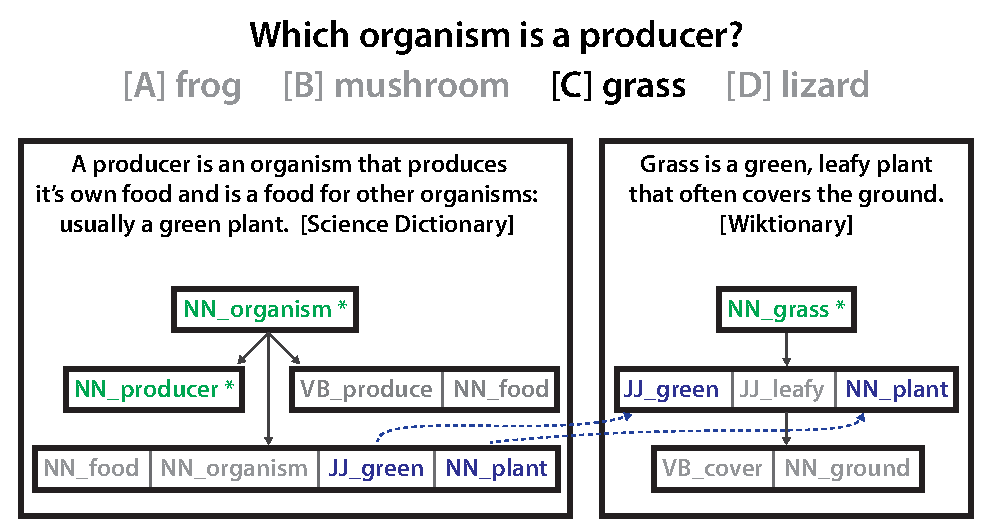
\includegraphics[width=75mm]{example_tig_producer2.pdf}
%\vspace{-2mm}
%\caption{ An example TAG path and justification rated as {\em good}. \note{TODO: Redraw figure with different line widths, closer to the original DOT file?}}
%%\caption{{\small An example of the alignments produced by the two discourse models.  The sequential model aligns pairs of consecutive sentences, capturing intersentence associations such as \emph{cider--apples}, and \emph{orchard--autumn}.  The RST model generates alignment pairs from participants in all (binary) discourse relations, capturing both intrasentence and intersentence alignments, including 
%%\emph{apples--orchard, cider--apples}, and \emph{cider--autumn}.}}
%% ms: I get the point, but there is value in brevity. Plus, maybe we should not use Bob as example :)
%%the intersentence alignments above along with intrasentence and multi-sentence alignments, including \emph{Bob--cider, apples--orchard}, and \emph{cider--autumn}.}}
%\vspace{-5mm}
%\label{fig:justificationTAGexample}
%\end{center}
%\end{figure}



\begin{table}[]
\small
\begin{tabularx}{\textwidth}{p{2.5cm}p{11cm}}
%\hline
%\multicolumn{2}{l}{EXAMPLE: Other} \\
\hline
% Question Info
Question & Which organism is a producer? (GR:5)     \\
Focus Word(s) &   (NN\_producer, 0.92) (NN\_organism, 0.08) \\
Answers & (A) frog  (B) mushroom   (C) grass    (D) lizard \\
\hline
% Correct Answer Info
Correct Answer &  grass \\
Focus Word(s) &   (NN\_grass, 1.00) \\
\multicolumn{2}{c}{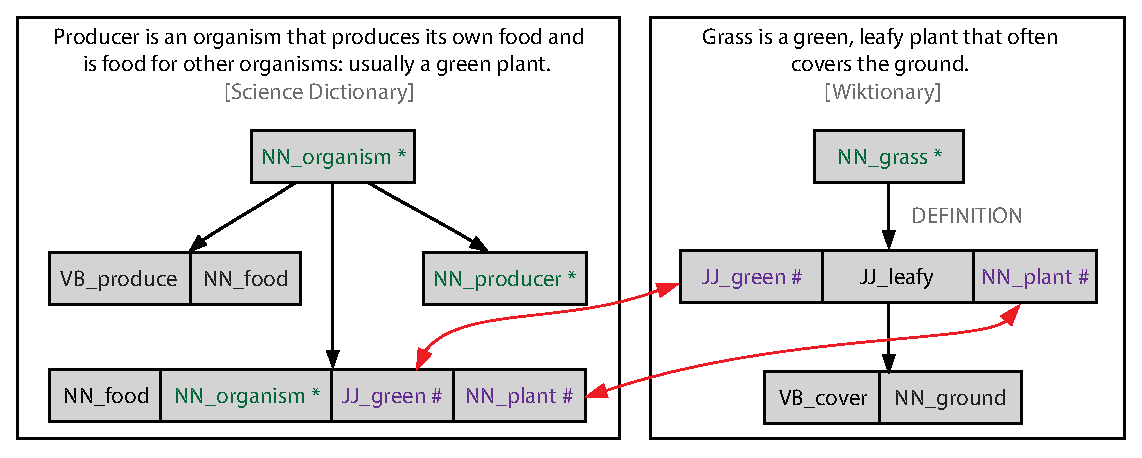
\includegraphics[width=115mm]{mainmatter/tacl2015-tig/tag_good_justification.pdf}}
\\
\hline
\end{tabularx}
\caption{{An example TAG and justification rated as {\em good}.  The two sentences connect on non-focus "other" shared words (e.g., \emph{green, plant}) which are not found in the question or answer, but which are highly related to the focus words. }} 

\label{ex:tagQsXs}
\end{table}






%
% Justification Examples - EXTRA
%
%\begin{table}[]
%\caption{{  Example of a TAG {\bf connected on answer focus} words. }} 
%\begin{tabularx}{\textwidth}{p{2.5cm}p{11cm}}
%%\hline
%%\multicolumn{2}{l}{EXAMPLE: Other} \\
%\hline
%% Question Info
%Question & What are the stages of development of an organism called? (GR:5)   \\
%Focus Word(s) &  (NN\_organism, 0.80) (NN\_stage, 0.13) (NN\_development, 0.07) \\
%\hline
%% Correct Answer Info
%Correct Answer &  Life cycle \\
%Focus Word(s) &  (NN\_cycle, 0.92) (NN\_life, 0.08) \\
%\multicolumn{2}{c}{\includegraphics[scale=0.5]{q58a1p2363connection.png}}\\
%\hline
%\end{tabularx}
%\label{ex:tagAns}
%\end{table}

%\begin{table}[]
%\caption{{  Example of a TAG {\bf connected on question and answer focus words}. (Somewhat more challenging focus word extraction, but we end up matching most of the words).  }} 
%\begin{tabularx}{\textwidth}{p{2.5cm}p{11cm}}
%%\hline
%%\multicolumn{2}{l}{EXAMPLE: Other} \\
%\hline
%% Question Info
%Question & Different types of organs that work together to perform a specific life function are called a(n) \_\_\_. (GR:5)   \\
%Focus Word(s) &   (VB\_work, 0.23) (VB\_perform, 0.23) (NN\_n, 0.23) (RB\_together, 0.09) (NN\_life, 0.07) (JJ\_specific, 0.06) (JJ\_different, 0.04) (NN\_function, 0.03) (NN\_organ, 0.01) \\
%\hline
%% Correct Answer Info
%Correct Answer &  organ system \\
%Focus Word(s) &   (NN\_system, 0.67) (NN\_organ, 0.33) \\
%\multicolumn{2}{c}{\includegraphics[scale=0.5]{q61a2p1104connection.png}}\\
%\hline
%\end{tabularx}
%\label{ex:tagQuest+Ans}
%\end{table}

%\begin{table}[]
%\caption{{  Example of a TAG connected only on answer focus words. Despite a non-ideal ranking of the question focus words, the system is able to lock onto this as a good justification of the correct answer.}} 
%\begin{tabularx}{\textwidth}{p{2.5cm}p{11cm}}
%%\hline
%%\multicolumn{2}{l}{EXAMPLE: Other} \\
%\hline
%% Question Info
%Question & Pots and pans are most often made from metal because \_\_\_. (GR:5)     \\
%Focus Word(s) &   (NN\_pot, 0.48) (NN\_pan, 0.48) (NN\_metal, 0.04) \\
%\hline
%% Correct Answer Info
%Correct Answer &  metals conduct heat well \\
%Focus Word(s) &   (NN\_heat, 0.44) (RB\_well, 0.44) (NN\_metal, 0.07) (VB\_conduct, 0.04) \\
%\multicolumn{2}{c}{\includegraphics[scale=0.5]{q100a3p908connection.png}}\\
%\hline
%\end{tabularx}
%\label{ex:tagXs}
%\end{table}

%\begin{table}[]
%\caption{{  {\bf Error example: Construction and Ranking vs Answer Selection:} Example of a question which requires {\bf complex inference}.  Our system aggregate sentences by connecting on {\bf question focus words as well as non-focus words}, to construct a good justification for the correct answer and rank it to the top of the justifications for that answer candidate. }} 
%\begin{tabularx}{\textwidth}{p{2.5cm}p{11cm}}
%%\hline
%%\multicolumn{2}{l}{EXAMPLE: Other} \\
%\hline
%% Question Info
%Question & In a food chain or web, the most efficient users of the Sun's energy are \_\_\_. (GR:5)     \\
%Focus Word(s) &   (NN\_chain, 0.23) (NN\_web, 0.23) (NN\_user, 0.22) (NN\_energy, 0.22) (NN\_food, 0.05) (NN\_sun, 0.03) (JJ\_efficient, 0.02) \\
%\hline
%% Correct Answer Info
%Correct Answer &  herbivores \\
%Focus Word(s) &   (NN\_herbivore, 1.00) \\
%\multicolumn{2}{c}{\includegraphics[scale=0.5]{q67a2p1connection.png}}\\
%\hline
%\end{tabularx}
%\label{ex:tagQsXsWrong}
%\end{table}
%
%
%\begin{table}[]
%\caption{{  {\bf Error example:} A similar example to the last one -- much of the time we're able to construct and rank very good TAGs (for a given answer candidate), but the last step -- selecting the best justification, is more sensitive to {\emph well connected answers} rather than {\emph good answers}.  Here the two aggregated sentences are {\bf connected on question focus words.}  }} 
%\begin{tabularx}{\textwidth}{p{2.5cm}p{11cm}}
%%\hline
%%\multicolumn{2}{l}{EXAMPLE: Other} \\
%\hline
%% Question Info
%Question & All organisms need food to survive. Which statement best describes the purpose of food for organisms? (GR:4)    \\
%Focus Word(s) &   (NN\_organism, 0.34) (NN\_organism, 0.34) (VB\_survive, 0.08) (NN\_food, 0.05) (VB\_need, 0.03) (NN\_food, 0.08) (NN\_purpose, 0.05) (NN\_statement, 0.03) \\
%\hline
%% Correct Answer Info
%Correct Answer &  Food provides energy for growth. \\
%Focus Word(s) &   (NN\_energy, 0.68) (NN\_growth, 0.16) (VB\_provide, 0.11) (NN\_food, 0.05) \\
%\multicolumn{2}{c}{\includegraphics[scale=0.5]{q19a3p2833connection.png}}\\
%\hline
%\end{tabularx}
%\label{ex:tagQsAsWrong}
%\end{table}
%
%
%
%\begin{table}[]
%\caption{{ {\bf Error example:} Another example of {\bf complex inference} that {\bf connects on other words}, in this case {\emph river}.  Again we're ranking this \todo{path} to the candidates for a given answer, but not selecting it out of the 4 multiple choice answers.  }} 
%\begin{tabularx}{\textwidth}{p{2.5cm}p{11cm}}
%%\hline
%%\multicolumn{2}{l}{EXAMPLE: Other} \\
%\hline
%% Question Info
%Question & Moving water was the most important factor in forming which of these? (GR:5)   \\
%Focus Word(s) &   (VB\_move, 0.68) (NN\_factor, 0.16) (NN\_water, 0.11) (JJ\_important, 0.05) \\
%\hline
%% Correct Answer Info
%Correct Answer &  the Grand Canyon \\
%Focus Word(s) &   (NN\_canyon, 0.67) (NN\_grand, 0.33) \\
%\multicolumn{2}{c}{\includegraphics[scale=0.5]{q33a0p57connection.png}}\\
%\hline
%\end{tabularx}
%\label{ex:tagXsWrong}
%\end{table}

The previous experiments demonstrate that our method performs well at identifying correct answers. But how well does it perform at the task of {\em justifying} those answers?
We evaluated justification performance for both the best baseline (IR) and the best performing TAG model that is independent of IR (i.e., 1G\textsubscript{CT} + 2G\textsubscript{CT}) .  Where TAG justifications took the form of the sentences being aggregated, justifications for the IR model were taken to be the highest-scoring short passages from each of the six knowledge bases.  As the IR model was tuned to a retrieval size of two sentences to maximize P@1 performance, each IR justification was two sentences in length.\footnote{Documents for the dictionary and flashcard corpora typically contained only a single sentence, and so answer justifications from these corpora are often shorter than two sentences.} To facilitate easy comparison, since the IR model provides six justifications (one from each knowledge base), we evaluate the top six scoring TAG justifications.  

Two of the authors independently rated the quality of the justifications. Any detected conflicts were resolved post hoc by the two annotators working together.
Answer justifications were rated on a four-point scale, based on their ability to provide a convincing justification to the user as to why a given answer choice was correct (see  Table~\ref{tab:justificationsIRexamples} for IR examples, and Figure~\ref{ex:tagQsXs} for a TAG example).   Justifications rated as {\em\bf good} describe the inference required to arrive at the correct answer.  Those rated as {\em\bf half} contained at least a portion of an explanation of the inference, but missed some critical aspect required to answer the question, like discussing producers but not consumers in Table~\ref{tab:justificationsIRexamples}. The two final ratings are for justifications that did not address the inference -- {\em\bf topical} justifications do not address the question but discuss a similar topic, where {\em\bf offtopic} justifications are unrelated to the question. 

%
% Justification performance
%
\begin{table}[t]
\small
\begin{center}
\begin{tabular}{p{20mm}cc}
\hline
\multicolumn{1}{l}{Rating} & \multicolumn{1}{c}{IR} & \multicolumn{1}{c}{TAG} \\%  & IR & TAG \\
\cline{2-3}
\hline
Good				&	45.3\%		& 56.7\%	 \\%	& 12.6\%		& 45.1\%	 \\
Half				&	34.9\%		& 20.7\%	 \\%	& 17.3\%		& 18.0\%	 \\
Topical			&	11.9\%		& 14.4\%	 \\%	& 17.2\%		& 18.4\% \\
Offtopic			&	7.9\%		& 8.2\%	 \\%	& 52.9\%		& 18.5\% \\

\end{tabular}
\caption{{ \emph{At least one} justification performance for both IR and TAG models, reflecting the highest rating attained by at least one of the top six justifications for a given question. }}%  Precision@6 performance reflects the overall proportion of each rating across all of the top six justifications. }} %  
\label{tab:justifications}

\end{center}
\end{table}

We evaluated the top-rated answer justifications using an {\bf at least one} method.  With this method, performance reflects the highest rating attained by \emph{at least one} of the six justifications for a given question. For example, for a question to be classed as {\em good}, at least one of the six answer justifications must be rated as {\em good}.  \emph{At least one} answer justification performance is listed in Table~\ref{tab:justifications}. For the TAG model, 56.7\% of the questions had at least one justification rated as {\em good}, outperforming IR justifications by 11.4\% (absolute).  


This experiment supports our original intuition that justifications must be aggregated from multiple resources. While the small window of sentences from the IR model is sufficient to justifiably answer many questions, a large number of questions require knowledge to be aggregated from {\em non-adjacent} sentences within a given corpus, or from sentences in different corpora altogether, to compose convincing answer justifications.  While the IR model leaves many of these questions with only partial justifications (34.9\% of justifications are rated as {\em half}), the TAG model  is able to aggregate sentences from multiple sources, and finds complete {\em good} justifications for many of the questions only partially answered by the IR model.


\subsubsection{Ablation Studies}
\label{sec-cl2017:controls}
To verify the contribution of the components of our system, we include the following ablation studies:
%\paragraph{How does the latent layer in the Ranking Perceptron affect performance?}
{\flushleft {\bf Latent Perceptron:}} The complete removal of the latent layer (i.e., using the average of all TAG scores to score the candidate answer, and performing perceptron updates with all TAGs) decreases the performance of the best performing TAG model (1G\textsubscript{CT} + 2G\textsubscript{CT}) from 42.88 to 35.43 P@1.  Alternatively, we experimented with using the sum of the TAG scores and the maximum TAG score as the candidate score, while still doing updates with all TAGs.  These configurations decreased performance to 34.46 and 38.09 P@1, respectively. This demonstrates the importance of modeling justification quality as a latent variable.

%\paragraph{How do the focus words impact performance?}
{\flushleft {\bf Focus Words:}} Focus words are used both to find relevant sentences to aggregate into answer justifications, as well as to characterize those justifications when expressed as TAGs. Replacing focus words with uniform weights for all content words (NN, VB, JJ) in a question reduces performance of the 1G+2G model from 38.69 to 33.89 P@1.  For the connection-type-aware model (1G\textsubscript{CT} + 2G\textsubscript{CT}), performance decreases from 42.88 to 40.03 P@1. This supports our observation that science exam questions contain several layers of information (e.g., the underlying question, and the example the question is grounded in), each contributing different utility to the QA process. 

%\paragraph{How does the graphlet structure impact performance?}
{\flushleft {\bf Graphlet Structure:}}  Graphlets segment sentences based on clausal and prepositional boundaries to facilitate evaluating how well two sentences connect using structures larger than a word but more fine-grained than the entire sentence.  
In other words, graphlets are the key structure in our representation of answer justifications because they drive both intra- and intersentence connections in a TAG. 
Eliminating this structure (i.e., considering each sentence as a bag of words, which is equivalent to a graphlet with a single nugget)
substantially reduces the performance of the 1G + 2G model from 38.69 to 28.90 P@1 and the performance of the 1G\textsubscript{CT} + 2G\textsubscript{CT} model from 42.88 to 28.08 P@1. 

\begin{comment}

\begin{figure}
\centering
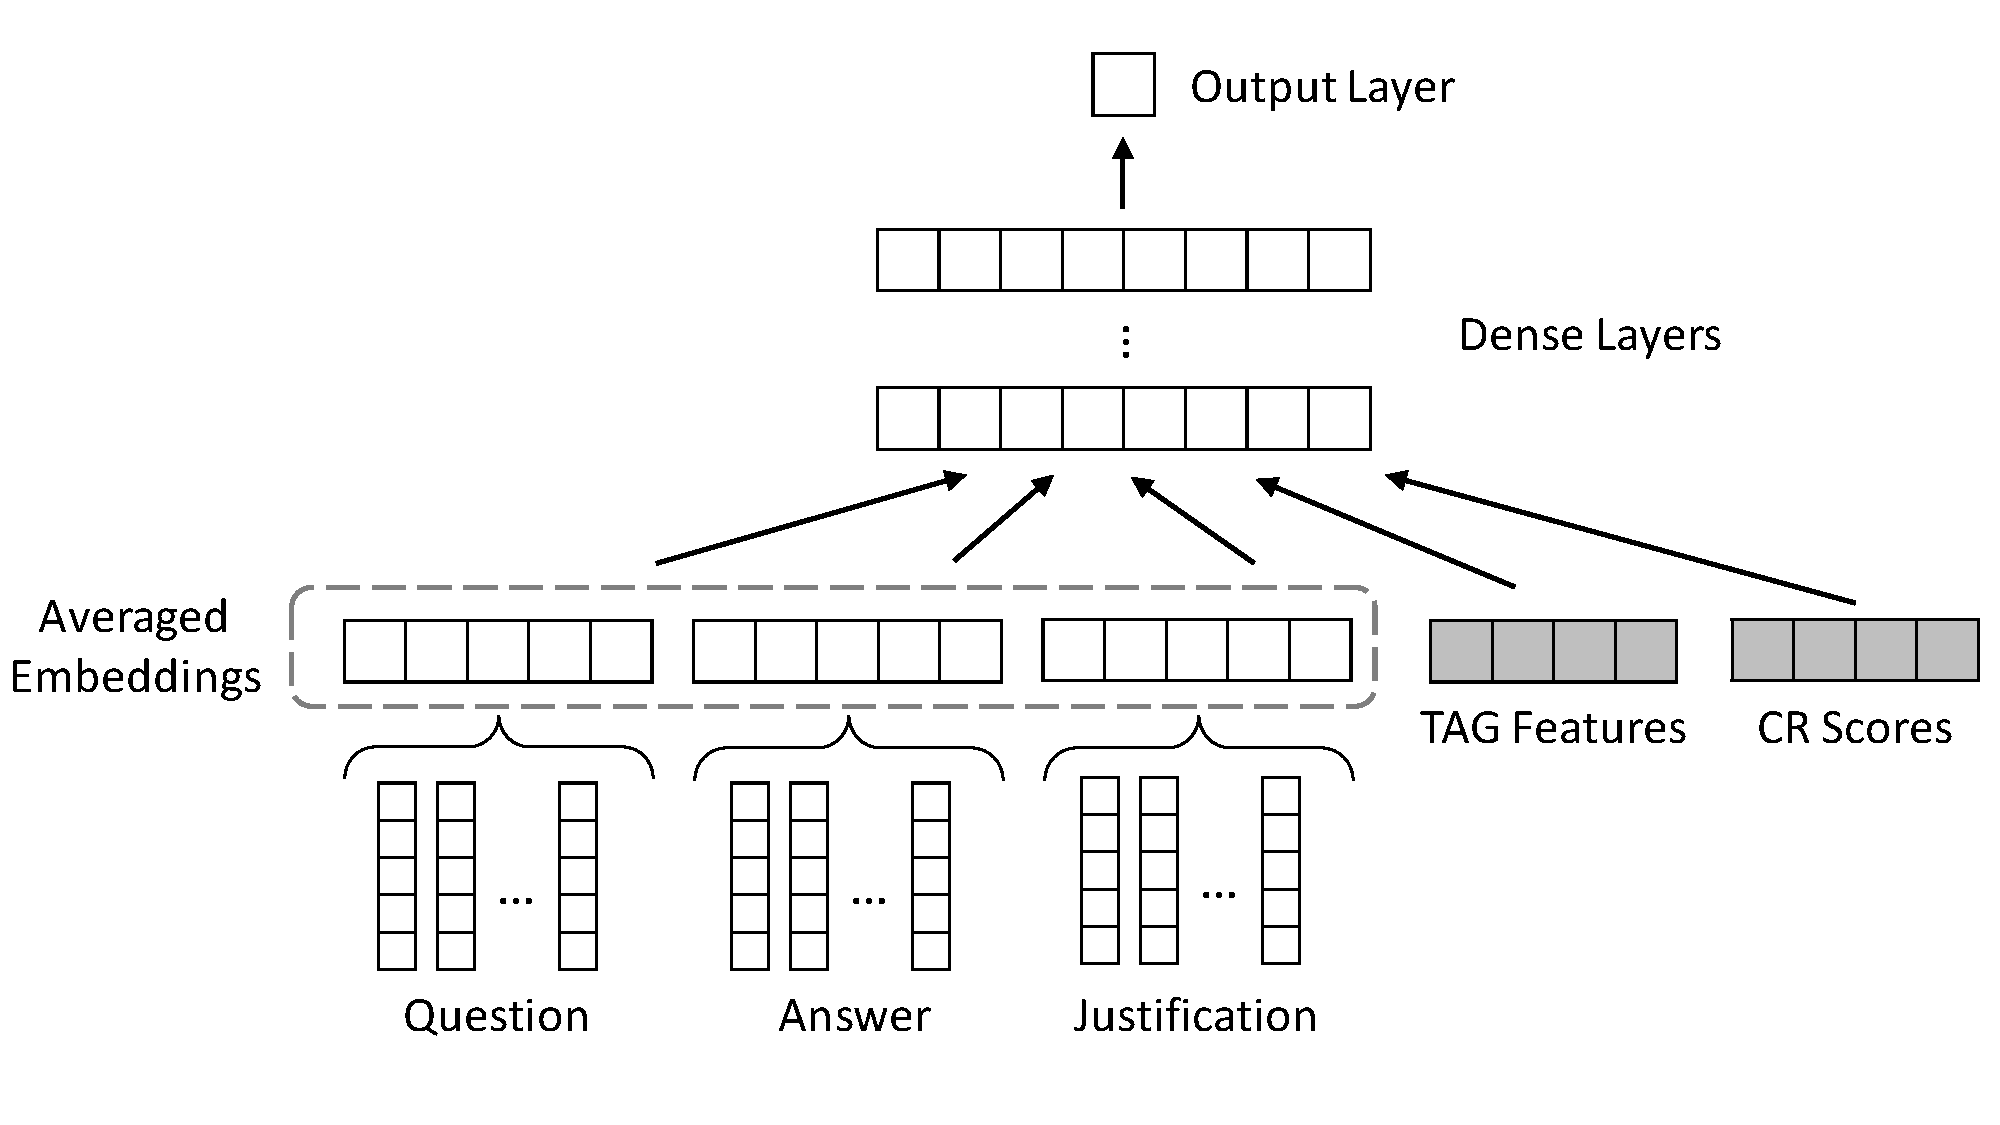
\includegraphics[width=0.8\textwidth]{mainmatter/tacl2015-tig/tagNNArch2scores.pdf}
\caption{The architecture for the neural network variation of our TAG system. We use a fully-connected feed-forward network which takes as input the content words (i.e., nouns, verbs, and adjectives) from the question, candidate answer, and corresponding justification.  For each of these, we create a composite vector by averaging the embeddings of the individual words.  We then concatenate these three composite vectors, as well as the TAG features and the IR scores, to form the input layer to the network. The output of the network is a single, real-valued score for the candidate answer justification.}
\label{fig:nn_arch}
\end{figure}


\subsection{From Latent Perceptron to Latent Neural Networks}
\label{sec-cl2017:nn}

Neural networks (NNs) have recently received much attention in many NLP tasks and have been shown to be quite effective in certain question answering tasks~\citep{Iyyer2014,bordes2014question,bordes2015large,Iyyer2015,wang2015long,dong2015question,yih2015semantic,he2016pairwise,suggu2016deep}.  To determine if a deep learning approach would benefit our system, we explored providing our text aggregation graph features and the information retrieval scores to a neural ranking architecture.  Under this framework we were also able to straightforwardly experiment with including vectorized representations (i.e., embeddings) of the question, candidate answer, and corresponding justification, in hopes of accommodating some of the lexical variation in natural language.

Neural network systems have varied dramatically in terms of their primary architecture (i.e., feed-forward, convolutional, recurrent, etc.) as well as their shape (number of hidden layers, number of nodes in a given layer, etc.).  Recently, however, \citet{Iyyer2015} found that in their QA task, a simple network which \emph{averaged} the word embeddings of the questions and the answer candidates outperformed a much more complex tree recurrent NN.  
\citet{chen2016acl} have recently validated this observation in a different QA task.
We based our NN on this simpler system, adapting it to our task by including not only an averaged vector for the question and answer, but also an averaged vector for the answer justification.  Additionally, we include our connection-type aware structural TAG features (cf., Table \ref{tab:features}) and the information retrieval (IR) features in the network input.  The network architecture is shown in Figure \ref{fig:nn_arch}.

For learning, we use the hinge ranking loss function \citep{collobert2011natural} and update using stochastic gradient descent (SGD).  During training, for each question we pair the correct answer candidate with each of the incorrect candidates, creating three pairs.  For each of these pairs, we score both the correct answer candidate and the incorrect answer candidate and then compute the loss:
\begin{equation}
L = \max (0, m - F(q,a_{correct}) + F(q,a_{incorrect}))
\end{equation}
where $F(q,a_{correct})$ is the score of the correct answer candidate, $F(q,a_{incorrect})$ is the score of the incorrect answer candidate, and $m$ is the margin.


There are two important aspects of the proposed architecture:
\begin{enumerate}
\item[a)] The latent layer, i.e., identifying good justifications to use for a given answer, which we implement by modifying SGD to keep track of the latent aspect.  Specifically, to maintain the latent variable aspect of our ranking perceptron in our ranking neural network, we adapt Equation \ref{eq:F} to use a feed-forward pass through the network to determine the score of a given TAG (rather than the inner product of the features and the parameter vector), and continue to use the implementation of $P$ that uses only the TAG with highest score.  In this way, for each pair of candidate answers we have two justifications (one for the correct answer and one for the incorrect), and so perform a model update (i.e., backpropagation) for each.
\item[b)] The combination of embeddings with explicit features that come from the IR system and the TAG features.  This strategy of mixing latent and explicit features has been demonstrated to be successful in other NLP tasks \citep{chen2014fast,suggu2016deep}.
\end{enumerate} 

Despite their advantages, neural networks have many hyperparameters which need to be tuned.  Continuing the inspiration of \citet{Iyyer2015}, we lightly turned the network on development, both in terms of network shape as well as additional parameters.  Doing so, we arrived at a network which has a single dense layer with length 100 followed by the output layer of length one.\footnote{We experimented with some deeper networks and several hidden layer sizes (both larger and smaller).} 
For our word embeddings, we used a recurrent neural network language model \citep[RNNLM;][]{mikolov10,mikolov13} trained over a concatenation of all of our in-domain elementary science resources (i.e., the study guides, flashcards, and dictionaries) to generate embeddings with 200 dimensions.\footnote{We also experimented with using embeddings trained over English Gigaword \citep{graff2003english} since the resource is much larger and would potentially yield more robust word representations.  However, we found that the performance was consistently worse, which we suspect is due to the difference in the domains.}  


All network nodes use the sigmoid activation function, which performed better and was more stable to variations in the hyperparameters than the rectified linear unit activation.  Additionally, we used an L2 regularization of 1.0 and a dynamic learning rate which began at 1.0 and decayed by half each time the performance on validation decreased.  Though we experimented with dropout, there did not not seem to be a consistent improvement, so our final models do not include it.    
We used 50 epochs for training with early stopping if the validation performance decreased and failed to regain its previous best after 10 epochs.  Similar to the perceptron, we found that the network performance varied with the random seed.  To mitigate the effects of this variation, we report scores from an ensemble of five networks, each with a different random seed, where the trained networks each voted for a single answer choice, splitting their vote only in the event of a tie.


\begin{table*}
\small
\begin{center}
\begin{tabular}{p{0.3mm}p{45mm}ll}
%\multicolumn{1}{l}{ } & \multicolumn{1}{l}{ } & \multicolumn{1}{l}{ } & \multicolumn{1}{l}{P@1}  & \multicolumn{1}{l}{MRR} \\

\# & Neural Network Models  & P\@1 & MRR   \\
% IR - 40.74
% IR + CL + embed - 41.82
% IR + embed - 38.1
% IR + CL - 40.52
% CL - 39.72

\hline
1 & IR				&  40.74\%  & 62.56\%  \\
2 & IR + TAG 		&  40.52\%  & 62.48\% 	\\
3 & IR + embeddings		&  38.74\%  & 61.61\%  	\\
4 & IR + TAG + embeddings	&  41.82\%  & 63.11\%	\\
\end{tabular}
\caption{Performance of the Latent Ranking Neural Network models.  Models with \emph{IR} include the information retrieval scores as input, models with \emph{TAG} use the features from the best performing TAG model (1G\textsubscript{CT}+2G\textsubscript{CT}), and models with \emph{embeddings} include an average embedding for each of the question, the answer, and the text from which the justification graphlet was derived.  Significance tests were performed using bootstrap resampling with 10,000 iterations, but none of the differences between the neural network models and the IR baseline were significant.}
\label{tab:nnresults}
\end{center}
\end{table*}

\paragraph{Neural Network Results}
\label{sec-cl2017:nnresults}


The final performance for the neural network variants of our proposed system as well as the IR baseline are shown in Table \ref{tab:nnresults}.  Once again, we observe that the performance of the combined model (IR + TAG + embeddings, line 4) is better than the performance of the IR model by itself (line 1) or IR + embeddings (line 3). However, here this difference is not significant.  This suggests that representing the justification as a simple bag of words with latent feature representations is not as effective as representing them with features derived from the structure of the text aggregation graph, even with the non-linear capabilities of the neural network.

Additionally, we find that the neural network variants perform worse overall than the latent ranking perceptron models and the voting ensemble (cf., Table \ref{tab:combinedmodels}).  This could be due to the fact that the TAG and IR features we are supplying to the neural network are already abstracted many levels from raw text inputs, and so the NN approach benefits less from the non-linearity of the NN.  Another likely reason for the NN performing worse than the perceptron is that neural architectures need larger quantities of training data in order to properly generalize.  Notably, in the recent Allen Institute for Artificial Intelligence Kaggle challenge\footnote{\url{https://www.kaggle.com/c/the-allen-ai-science-challenge}}, a large contest with 170 participating teams, which also required answering multiple choice elementary and middle school science questions, none of the top-performing participants obtained better results with neural networks. The participants' analyses suggested that this is largely due to a lack of training data.  Finally, the space of possible neural network architectures is large, and the network we report here is fairly simple.  While it could be the case that given a more complex architecture (i.e., with a recurrent or convolutional network, optimizers, and learned rather than pre-trained embeddings) we could obtain even higher numbers than those reported here, with complex architectures, issues resulting from the limited training data would likely be worsened. We leave that exploration to future work.

\paragraph{Incorporating Embeddings into the Perceptron}
Though the embedding-based neural architecture (as implemented) was not successful, following a reviewer suggestion we also experimented with adding the precomputed text embeddings as additional features for the latent ranking perceptron.  In this way, the feature vector for each TAG, $\Phi(x)$, contains the original features as well as an averaged embedding for each of the question, answer, and justification texts.  This provides an additional 600 features, as we are using 200-dimensional embedding vectors.  We included these extra features in our best performing single TAG model, the connection-type aware 1G+2G model shown in Table \ref{tab:combinedmodels}, line 5.  The resulting model performed worse (39.36\% P@1 compared to 42.88\% P@1 without the embeddings). 
This shows that, while distributed representations of words have many benefits (including robustness to lexical variation), their incorporation into a learning model is not necessarily trivial, and we leave that study to future work.

\end{comment}
\section{Discussion}
\label{sec-cl2017:discussion}

To further characterize the performance of our QA approach, we address the following questions: 


%%
%% Comparison with TableILP
%%
%\begin{table}[t]
%\caption{{ Comparison with other models }} % 
%\small
%\begin{center}
%\begin{tabular}{lccc}
%%\cline{2-3}
%%\begin{tabular}{p{20mm}cc}
%\hline
%\multicolumn{1}{c}{Model} & \multicolumn{1}{c}{Questions} &\multicolumn{1}{c}{P@1} \\
%\cline{2-3}
%\hline
%CR $\cup$ (1G\textsubscript{CT} + 2G\textsubscript{CT}) $\cup$ 3G\textsubscript{CT} 			 	& 1000		&	44.6\%	\\
%Khashabi et. al (2016)																				& 200 		&	45.6\%	\\
%
%\end{tabular}
%\label{tab:tableilp}
%\end{center}
%\end{table}

{\flushleft {\bf How does performance compare with methods using manually constructed knowledge bases?}} The TAG system automatically aggregates sentences from six free-text corpora first by building graphlets from those sentences using syntactic dependencies, then connecting those graphlets together into multisentence text aggregation graphs that are then used to both answer questions and provide a compelling human-readable justification for the selected answers.  Recently, Khashabi et al. \citeyear{Khashabi2016QuestionAV} demonstrated that graphs for elementary science QA can also be constructed using a semistructured knowledge base of tables.  In this formalism, dozens of themed tables are manually or semi-automatically constructed, each around a particular theme.  A table's theme is encoded in it's columns, i.e., a table for the color of objects contains two rows, one for the object of interest (e.g., ``leaf''), and another for it's color (e.g., ``green''), while separate instances (e.g., leaf -- green, trunk -- brown) are encoded as different rows.  Each table has between two and five columns.  

The TableILP algorithm answers questions by chaining facts between different table rows, starting from a row that contains question terms, then traversing to a new table row that contains some lexical overlap with the previous row(s), until answer terms are found.  The TAG and TableILP systems are conceptually similar, with the central differences being: (1) The TableILP table row is roughly equivalent to a TAG graphlet with flat structure, and limited to 2--5 information nuggets containing only single terms, (2) TAG graphlets are read automatically from free text corpora, where TableILP tables are largely manually constructed, with methods to automate this construction being actively developed, and (3) the traversal algorithms are different, with TableILP graph building being modelled as an integer linear programming (ILP) problem which finds paths that maximize QA performance.  

The TableILP system reported by Khashabi et al. \citeyear{Khashabi2016QuestionAV} contains 69 tables containing a total of 7,600 rows, with 64 of these tables (approximately 5,000 rows) designed around material in the study guides and a development corpus, and the remaining 2,600 rows distributed amoung 4 automatically constructed tables.  On a corpus of 200 questions drawn from the 1,000 questions used here, TableILP achieved a score of 45.6\% P@1\footnote{We wish to thank Khashabi et al. \citeyear{Khashabi2016QuestionAV} for providing us with this performance figure.}, compared to the 44.6\% P@1 from the best-performing TAG model in Table~\ref{tab:combinedmodels}. The performance difference between these systems is likely not statistically significant.\footnote{We did not have access to system output. However, in our experiments on this dataset, we observed that only differences in P@1 scores of 3\% or higher (absolute) tend to be statistically significant at $p < 0.05$.}

We view these systems as complementary, converging, and with each capable of exploring different aspects of graph-based inference for science QA.  While the TAG focuses on automatically building graphs from free text, this is currently a challenging and noisy process, and as we have shown in Table~\ref{tab:pathlength} and Fried et al.~\citeyear{fried2015higher}, highly susceptable to inference drift as the amount of information required to be aggregated becomes large.  On the other hand, building graphs from manually constructed knowledge bases allow us to investigate the graph-building process in isolation, reducing inference drift due to noise, and further moving this area forward.  

%
% Performance by grade level
%
\begin{table}[t]
\caption{{ Precision@1 by grade level. }} % 
\small
\begin{center}
\begin{tabular}{lccc}
%\cline{2-3}
%\begin{tabular}{p{20mm}cc}
\hline
\multicolumn{1}{c}{Grade Level} & \multicolumn{1}{c}{Questions} &\multicolumn{1}{c}{CR} & \multicolumn{1}{c}{TAG}  \\
\cline{2-3}
\hline
Grade 3 	& 60		&	28.3\%		& 49.2\%	\\
Grade 4		& 69 	&	50.7\%		& 41.3\%	\\
Grade 5		& 871	&	40.2\%		& 42.6\%	\\

\end{tabular}
\label{tab:gradelevel}
\end{center}
\end{table}


{\flushleft {\bf How does performance vary by grade level?}} The question corpus contains third, fourth, and fifth grade questions.  A human with a level of knowledge equivalent to a fourth grade science student might be expected to show better performance for the simpler third grade questions, and decreasing performance as question difficulty increases from fourth to fifth grades.  Table~\ref{tab:gradelevel} shows P@1 performance by grade level for both the CR and best performing TAG model (1G\textsubscript{CT} + 2G\textsubscript{CT}).  The TAG model shows decreasing performance as question difficulty increases, dropping from 49\% for third grade questions to 42\% for fourth and fifth grade questions.  The CR baseline, however, displays a qualitatively different pattern, with a peak performance of 51\% for fourth grade questions, and {\em near chance} performance for third grade questions. 
We believe that observing such a pattern in performance may suggest that the TAG model is a closer approximation of human inference than the baseline based solely on information retrieval.  Here, the relatively small number of third and fourth grade questions prevents us from drawing any conclusions, but suggests that crafting question sets to allow evaluating the distribution of performance by grade level may provide a further measure of comparison between human and machine performance. 



%
% Justification performance by knowledge resource
%
\begin{table}[t]
\caption{{ Most useful knowledge resources for justifications classified as "good".}}
\small
\begin{center}
\begin{tabular}{lccc}
%\cline{2-3}
%\begin{tabular}{p{20mm}cc}
\hline
\multicolumn{1}{l}{Resource} & \multicolumn{1}{c}{Sentences} &\multicolumn{1}{c}{CR} & \multicolumn{1}{c}{TAG}  \\
\cline{2-3}
\hline
Barrons SG 			& 1,200		&	39.3\%		& 43.0\%	\\
Flashcards			& 283		&	16.2\%		& 8.2\%	\\
Teacher's Guide		& 302		&	7.1\%		& 7.0\%	\\
Virginia SG			& 1,314		&	9.1\%		& 9.2\%	\\
Science Dictionary	& 733		&	20.8\%		& 17.8\%	\\
Simple Wiktionary	& 17,473		&	7.5\%		& 14.8\%	\\

\end{tabular}

\label{tab:justificationknowledgeresources}
\end{center}
\end{table}

{\flushleft {\bf Which knowledge resources are generating the most useful answer justifications?}} Shown in Table~\ref{tab:justificationknowledgeresources}, the Barron's Study Guide (SG) contributes more of the \emph{good} justification sentences than any other source, followed by the science dictionary, then the other resources.  Interestingly, the Simple Wicktionary contributes the fewest sentences to the \emph{good} justifications for the CR system (7.5\%), but for the TAG system it is the third largest contributor (14.8\%).  That is, while the CR system is typically unable to find a \emph{good} justification from the Wiktionary, likely owing to it's general nature, the TAG system is able to successfully aggregate these sentences with sentences from other domain-specific sources to build complete justifications.

The vast majority of the \emph{good} justifications generated by the TAG system are aggregates from non-adjacent text: 67\% of the justifications aggregate sentences from \emph{different} corpora, 30\% aggregate non-adjacent sentences within a \emph{single} corpus, while only 3\% of \emph{good} justifications contain sentences that were adjacent in their original corpus. 
This is clear evidence that information aggregation (or fusion) is fundamental for answer justification.


{\flushleft {\bf How orthogonal is the performance of the TAG model when compared to CR?}} Both the TAG and CR models use the same knowledge resources, which on the surface suggests the models may be similar, answering many of the same questions correctly.  The voting models in Table~\ref{tab:combinedmodels} appear to support this, where combining the TAG and CR models increases performance by just under 2\% P@1 over the best-performing TAG model.  To investigate this, we conducted an orthogonality analysis to determine the number of questions both models answer correctly, and the number of questions each model uniquely answers correctly.

Comparing the TAG (1G\textsubscript{CT} + 2G\textsubscript{CT}) and CR models, nearly half of questions are answered correctly by one model and incorrectly by the other.  When combined into a two-way voting model, this causes a large number of ties -- which, resolved at chance, would perform at 42\%, with ceiling performance (i.e., all ties resolved correctly) at 60\%.  This indicates that while the TAG and CR models share about half of their performance, each model is sensitive to different kinds of questions, suggesting that further combination strategies between TAG and CR are worth exploring.


\section{Error Analysis}
\label{sec-cl2017:erroranalysis}

%
% Connection Types in Correct vs Incorrect Answers
%
\begin{table}[t]
\small
\label{tab:errorconnectiontypes}
\begin{center}
%\begin{footnotesize}
%\begin{tabular}{lcc}
%\cline{2-3}
\begin{tabular}{ccc}
\hline
\multicolumn{1}{l}{Connecting Categories} & \multicolumn{1}{c}{Correct} & \multicolumn{1}{c}{Incorrect}  \\
\cline{2-3}
\hline
1				&	31.0\%		& 57.6\%	\\
2				&	56.3\%		& 39.4\%	\\
3				&	12.7\%		& 3.0\%	\\
\end{tabular}
%\end{footnotesize}
\caption{{ Proportion of good justifications with a given number of connecting word categories (Q, A, X) for both correct and incorrect answers. (Top 6) }}
\end{center}
\end{table}

At a high-level, our sentence aggregation model can be thought of as a system for building and evaluating answer justifications.  When questions are answered incorrectly, it is unclear whether the system was unable to \emph{build} a good justification for the correct answer, or unable to \emph{detect} a good justification that was successfully built.  To examine this, in addition to evaluating justification quality for correct answers, we also evaluated the top six justifications for 100 questions that the TAG system answered incorrectly.  We investigated the type of TAG patterns in the correct justifications  (from Section \ref{sec-cl2017:characterizing}), as well as the kinds of inference required for questions that were answered incorrectly.  In addition, we conducted a large open-ended error analysis and identified several broad classes of issues that contribute to poor system performance.\footnote{Our current focus word extractor is not yet well suited to complex multisentence questions. While the question corpus as a whole consists of 62\% single-sentence questions, 25\% two-sentence questions, and 14\% questions which are three sentences or longer, we elected to focus on shorter single-sentence questions for this error analysis whenever possible.  As a result, 96\% of the questions analyzed were single-sentence and 4\% were two-sentence.}

{\flushleft {\bf What patterns of lexical overlap do we observe in justification sentences?}}
We begin with an encouraging result. For questions that were answered incorrectly, nearly half (45.1\%) contain at least one \emph{good} justification within the top 6 for the correct answer.  This suggests that the current model is much better at generating and broadly ranking justifications than it is at the final step -- pushing the correct justification from the top 6 to the top position.  This result suggests that the TAG model may benefit from an improved ranking model. For example, while we currently use lexicalization to model TAG structures and quantify the overlap between candidate TAGs and the question, none of the features used by the ranking perceptron are explicitly lexicalized. 
%We explored some neural network variants of our models in Section \ref{sec-cl2017:nn}, which were better able to incorporate lexicalization, but did not see a performance gain.  These models can be extended in future work, however, to see if it is ultimately possible to make use of this lexicalization.


Further, for questions answered correctly, the \emph{good} justifications in the top 6 tend to connect on several of the three lexical overlap categories (i.e., question focus words, answer focus words, other shared non-focus words).  Table \ref{tab:errorconnectiontypes} shows that for questions answered correctly, in 69\% of cases good justifications are connected on 2 or 3 lexical overlap categories.  
Conversely, for questions that are answered incorrectly, the \emph{good} justifications are far more likely to contain sentences that only connect on a single lexical overlap category (57.6\% vs 31.0\% for questions answered correctly). 
This suggests that while less lexically connected answer justifications are not necessarily less numerous or of lower quality, they are much more challenging to detect given our current connectivity-centered features.  That is, the current features are very good at detecting well connected answer justifications, which correlate with good answers, but the features aren't able to directly detect good answer justifications, which is a more challenging theoretical problem.




%
% Knowledge Types
%
\begin{table}[t]
\small
\begin{center}
\begin{tabular}{lccc}

%\cline{2-3}
%\begin{tabular}{p{20mm}cc}
\hline
\multicolumn{1}{c}{} & \multicolumn{1}{c}{Good} &\multicolumn{1}{c}{No Good} & \multicolumn{1}{c}{}  \\
\multicolumn{1}{l}{Inference Type} & \multicolumn{1}{c}{Justification} &\multicolumn{1}{c}{Justification} & \multicolumn{1}{c}{Overall}  \\

%\cline{2-3}
\hline
Retrieval 			& 58\%		&	23\%		& 39\%	\\
General Inference	& 29\%		&	43\%		& 37\%	\\
Model-Based			& 13\%		&	34\%		& 25\%	\\
\hline
\end{tabular}
\caption{{  A summary of the inference type necessary for incorrectly answered questions.  The summary is broken down into three categories: incorrectly answered questions with a good justification in the top six, incorrectly answered questions without a good justification in the top six, as well as the overall proportions across these two conditions. }} 
\label{tab:knowledgetype}
\end{center}
\end{table}

{\flushleft {\bf Is it harder to detect justifications for certain kinds of inference? }}
We predict that questions requiring more challenging kinds of inference as identified by \citet{clark:2013}, like model-based or general inference questions, are likely more difficult for the TAG system to answer than simpler retrieval-based questions. 
Following the criteria described by Clark et al., we classified the 100 questions in the error analysis based on the inference type required to answer them correctly. 
This analysis, shown in Table~\ref{tab:knowledgetype}, suggests that it is much more challenging to detect \emph{good} justifications for questions that contain challenging inference.  Where 58\% of retrieval-based questions contained a \emph{good} justification within the top 6, this decreased to 29\% for questions requiring general inference, and to 13\% for questions requiring complex model-based reasoning.  Taken in conjunction with our analysis of lexical overlap categories, this suggests that good justifications for complex inference may tend to be less lexically connected, and thus more challenging to detect with our current framework. This suggests important avenues for future work.

\subsection{Broader Error Classes}

\begin{table}[!tb]
\small
\begin{center}
\begin{tabular}{lccc}

%\cline{2-3}
%\begin{tabular}{p{20mm}cc}
\hline
\multicolumn{1}{c}{} & \multicolumn{1}{c}{Good} &\multicolumn{1}{c}{No Good} & \multicolumn{1}{c}{}  \\
\multicolumn{1}{l}{Error Class} & \multicolumn{1}{c}{Justification} &\multicolumn{1}{c}{Justification} & \multicolumn{1}{c}{Overall}  \\

%\cline{2-3}
\hline
\textbf{FOCUS WORDS}  	& 		&		& 	\\
%Focus Word - Question - Major Issues 	& 	27\%		&	30\% 	& 	29\%	\\
%Focus Word - Question - Minor Issues 	& 	22\%		&	16\%		& 	19\%	\\
%Focus Word - Answer - Major Issues 		& 	11\%		&	7\%		& 	9\%	\\
%Focus Word - Answer - Minor Issues 		& 	9\%		&	25\%		& 	18\%	\\
Focus Word --- Question 					& 	49\%		&	46\% 	& 	48\%	\\
Focus Word --- Answer 						& 	20\%		&	32\% 	& 	27\%	\\
Focus Word --- Answer Lists 				& 	7\%		&	5\%		& 	6\%	\\
Focus Word --- Compounds/Collocations 		& 	9\%		&	16\%		& 	13\%	\\
%Focus Word - Answer-type words  			& 	2\%		&	5\%		& 	4\%	\\
\hline
\textbf{NOISE IN THE KNOWLEDGE BASE}		& 			&			& 	\\
Excessively Long Sentence (Chosen Ans) 	& 	33\%		&	9\% 		& 	20\%	\\
Excessively Long Sentence (Correct Ans) 	& 	13\%		&	4\% 		& 	8\%	\\
\hline
\textbf{COMPLEX INFERENCE}				& 			&			& 	\\
More Sentences Required 					& 	4\%		&	16\% 	& 	11\%	\\
Causal or Process Reasoning 				& 	27\%		&	30\%		& 	29\%\\
Quantifiers	 							& 	4\%		&	23\% 	& 	15\%	\\
Negation	 								& 	2\%		&	9\% 		& 	6\%	\\
\hline
\textbf{MISCELLANEOUS}					& 			&			& 	\\
Semantic Cluster Matching				& 	16\%		&	5\%		& 	10\%\\
Coverage of Knowledge Bases				& 	4\%		&	36\%		& 	22\%\\
Other									& 	29\%		&	9\%		& 	18\%\\
\hline
\end{tabular}
\caption{{  A summary of the classes of the errors made by the system. On any given question, more than one error may have been made. The summary is broken down into three categories: incorrectly answered questions with a good justification in the top six, incorrectly answered questions without a good justification in the top six, as well as the overall proportions across these two conditions.}} 
\label{tab:errorclasses}
\end{center}
\end{table}

To expand on the above two issues, we conducted a broader, open-ended error analysis, and identified six main error classes made by the system: focus word failures, noise in the knowledge base, complex inference, semantic cluster matching, coverage of the knowledge bases, and other errors.  The distribution of these errors is shown in Table \ref{tab:errorclasses} and detailed below.

% -------------- FW - MAJOR
 
\begin{table}[]
\begin{footnotesize}
\begin{tabularx}{\textwidth}{p{2.5cm}p{10cm}}
\hline
\multicolumn{2}{l}{Focus Words --- Question} \\
\hline
% Question Info
Question 		& What type of simple machine is Bruce using as he opens a twist top bottle of soda? (GR:5) \\
Focus Word(s) 	& (NN\_bruce, 0.22) (VB\_open, 0.22) (NN\_twist, 0.22) (JJ\_top, 0.22) (NN\_bottle, 0.05) (NN\_soda, 0.03) (NN\_machine, 0.02)		     \\
\textbf{Issue}	& The concept the question is testing is embedded in a complex example that the focus word extractor is only partially able to suppress. Here, the most critical word for the inference is \emph{twist}, but some example words (\emph{bruce, open} and \emph{top}) are not suppressed, and receive the same weight as \emph{twist}. \\
 %which should be removed by the focus word extractor along with \emph{bottle} and \emph{soda}.}\\
\hline
\end{tabularx}
\end{footnotesize}
\caption{{  Example of failure to extract appropriate focus words from the question. }} 
\label{ex:majorfw}
\end{table}


{\flushleft {\bf FOCUS WORD ERRORS: }}
Extracting focus words from questions and answers can be difficult, as often these questions are grounded in complex examples.  Moreover, while examples can often be filtered out, sometimes they are necessary to the question. Within the larger category of focus word errors, we subdivided these errors into more specific categories: 

{\flushleft \emph{Question and Answer Focus Words: }}
We considered a question or answer to have focus word issues if either the words selected by the focus word extractor were not critical to the inference, or if the weights did not reflect the relative importance of each word to the inference.  An example of this can be seen in Table~\ref{ex:majorfw}.

{\flushleft \emph{Answer Choice Lists: }}
Candidate answers may not be single choices, but occasionally take the form of lists, as in the question \emph{which of the following organisms are decomposers?} and its correct answer \emph{worms, mushrooms, and insects}.  In these cases each list item for a given answer candidate must be independently verified for correctness, as incorrect lure answers often contain one or more correct list items.  The current system does not handle this type of complex problem solving method. 

{\flushleft \emph{Compounds/Collocations: }}
The current focus word extractor operates at the level of the word, and does not join noun--noun compounds or collocations, such as \emph{simple machine} or \emph{water cycle}.  This causes compounds to be split, with different focus weights assigned to each word.  This also adds noise to the inference process, as (for example) a justification sentence that contains \emph{simple} but not \emph{machine} is less likely to be on context. 
  

{\flushleft {\bf NOISE IN THE KNOWLEDGE BASE:}}
We included nearly all sentences contained in each of the five science-domain corpora.  While most of this is high-quality text, occasionally extremely long sentences are present (e.g., prefacing a chapter with a list of keywords).  These sentences can cause broad topic-level lexical connections between sentences that are only marginally related to each other, and are a source of noise in the justification building process.  



% -------------- LONGER CHAINS
 
\begin{table}[]
\begin{footnotesize}
\begin{tabularx}{\textwidth}{p{2.5cm}p{10cm}}
\hline
\multicolumn{2}{l}{Complex Inference --- More sentences required to construct a complete answer} \\
\hline
% Question Info
Question 		& Which of the following would result in a decrease in the polar bear population in the arctic? (GR:5) \\
Focus Word(s) 	& (JJ\_polar, 0.29) (NN\_population, 0.29) (NN\_arctic, 0.29) (VB\_result, 0.07) (NN\_decrease, 0.04) (NN\_bear, 0.02) \\
\textbf{Issue}	&  Requires additional graphlets, including that \emph{bears} eat \emph{fish}, \emph{eating} an animal makes you a \emph{predator} and it your \emph{prey}, and a decrease in \emph{prey} population also causes a decrease in \emph{predator} population.  Here, with a limited justification length of two sentences, the system is not able to construct a justification that includes all the crucial focus words, and all answer candidates are left with the same general justification fragment that includes the highest-weighted focus words. \\
\hline
% Correct Answer Info
Correct Answer 	&  a decrease in the fish population \\
Focus Word(s) 	&  (NN\_population, 0.80) (NN\_decrease, 0.13) (NN\_fish, 0.07) \\
Justification 	& A polar bear is a big, white bear that lives in the arctic. (Wiktionary)\\
 				& The population of a place is the people or animals that live there.  (Wiktionary)\\
\hline
% Chosen Answer Info
Chosen Answer 	& a decrease in the human population \\
Focus Word(s) 	& (NN\_population, 0.92) (NN\_decrease, 0.08) \\
Justification 	& A polar bear is a big, white bear that lives in the arctic. (Wiktionary)\\
 				& The population of a place is the people or animals that live there.  (Wiktionary)\\
\hline
\end{tabularx}
\end{footnotesize}
\caption{{  Example of a question that needs more than two sentences to answer. }} 
\label{ex:longerchains}
\end{table}

% -------------- CAUSAL REAS.
 
\begin{table}[]
\begin{footnotesize}
\begin{tabularx}{\textwidth}{p{2.5cm}p{10cm}}
\hline
\multicolumn{2}{l}{Complex Inference --- Causal or Process Reasoning} \\
\hline
% Question Info
Question & In the water cycle, which process occurs {\bf after} condensation? (GR:5)  \\
Focus Word(s) & (NN\_condensation, 0.75) (VB\_occur, 0.13) (NN\_water, 0.06) (NN\_cycle, 0.06)\\
\textbf{Issue}		& Requires knowing that the water cycle is a stage-like process that proceeds as follows: \emph{evaporation}, \emph{condensation}, \emph{precipitation}.  The focus word extractor does not currently detect causal or process markers, and as such the focus words for the question do not include \emph{after}. \\ 
\hline
% Correct Answer Info
Correct Answer &  Precipitation \\
%Focus Word(s) &  (NN\_precipitation, 1.00) \\
Justification 	& Condensation, in the water cycle, {\bf this step leads to} precipitation. (Science Dictionary)\\
 				& When the humidity reaches 100 percent it is very likely that some form of precipitation will occur, depending on the temperature. (Barrons SG)\\
\hline
% Chosen Answer Info
Chosen Answer & Evaporation\\
%Focus Word(s) &  (NN\_evaporation, 1.00)\\
Justification 	& When water vapor changes to liquid water it is called condensation. (Barrons SG)\\
 	& Evaporation is defined as the change of water from its liquid phase to its gaseous phase. (Barrons SG)\\
\hline
\end{tabularx}
\end{footnotesize}
\caption{{  Example of a question that requires reasoning over a causal structure or process. }} 
\label{ex:structure}

\end{table}


% -------------- QUANTIFIERS
 
\begin{table}[]
\begin{footnotesize}
\begin{tabularx}{\textwidth}{p{2.5cm}p{10cm}}
\hline
\multicolumn{2}{l}{Complex Inference --- Quantifiers} \\
\hline
%% Question Info
Question 		& Which of the following is a factor that will cause different species to compete {\bf less?} (GR:5)  \\
Focus Word(s) 	& (NN\_species, 0.50) (JJ\_less, 0.17) (VB\_compete, 0.13) (VB\_cause, 0.10) (JJ\_different, 0.07) (NN\_factor, 0.03)\\
\textbf{Issue}			&  Requires connecting the idea that a \emph{large} supply causes \emph{less} competition.  The focus word extractor does not currently detect quantifiers, and as such the focus words for the correct answer do not include \emph{large}. \\
\hline
%% Correct Answer Info
Correct Answer 	&  A {\bf large} supply of resources\\
Focus Word(s) 	&  (NN\_supply, 0.92) (NN\_resource, 0.08)\\
%Justification 	& Individuals in a species may compete with each other for food, mates, space, water, and shelter within their environment. (Barrons SG)\\
% 				&  A place's infrastructure is the basic public works such as roads, electricity \& water supply, and schools, that allow it to function.  (Wiktionary)\\
\hline
%% Chosen Answer Info
Chosen Answer & {\bf Lack} of space \\
Focus Word(s) &  (NN\_space, 0.92) (NN\_lack, 0.08)\\
%Justification 	& The energy from the sun heated the water and caused it to evaporate - change from liquid water to water vapor. (Barrons SG)\\
% 	& Individuals in a species may compete with each other for food, mates, space, water, and shelter within their environment. (Barrons SG)\\
\hline
\end{tabularx}
\end{footnotesize}
\caption{{  Example of a question that requires an understanding of the quantifiers in both the question and the answers. }} 
\label{ex:quantifiers}
\end{table}

% -------------- NEGATION
 
\begin{table}[]
\begin{footnotesize}
\begin{tabularx}{\textwidth}{p{2.5cm}p{10cm}}
\hline
\multicolumn{2}{l}{Complex Inference --- Negation} \\
\hline
% Question Info
Question & Which of the following is an example of a chemical change? (GR:5)  \\
%Focus Word(s) & (JJ\_chemical, 0.92) (NN\_change, 0.08)\\
\textbf{Issue}			&  Requires detecting negation in the graphlets.  The chosen answer justification contains negative evidence against itself. \\
\hline
% Correct Answer Info
Correct Answer &  Milk souring\\
%Focus Word(s) &  (NN\_souring, 0.67) (NN\_milk, 0.33)\\
Justification 	& Examples of chemical properties include the souring of milk and the ability to burn in the presence of oxygen. (Barrons SG)\\
 				& Evidence of a chemical change could be change in temperature, light, heat, or sound given off, or the formation of gasses. (Science Dictionary)\\
\hline
% Chosen Answer Info
Chosen Answer & Ice cream melting\\
%Focus Word(s) &  (NN\_melting, 0.80) (NN\_cream, 0.13) (NN\_ice, 0.07) \\
Justification 	& Melting of ice is a physical change, {\bf not a chemical change}. (Barrons SG)\\
 	& Melting is a process of an object changing from the solid state to the liquid state without a change in temperature. (Wiktionary)\\
\hline
\end{tabularx}
\end{footnotesize}
\caption{{  Example of a question that requires an understanding of negation. }} 
\label{ex:negations}

\end{table}



{\flushleft {\bf COMPLEX INFERENCE:}}
Despite the elementary-level of our question set, some questions require complex inference to be answered correctly (a recent analysis of a very similar elementary science question set indicated that as many as 77\% of questions required a form of complex inference to solve \citep{jansen-EtAl:2016:COLING}).  This may take the form of requiring longer sequences of graphlets to construct a complete answer justification, requiring an understanding of quantifiers or negation, or a complex inference process. 

{\flushleft \emph{More sentences required: }}
In our knowledge base, a sentence tends to capture a single step in some process. While two sentences are often sufficient to construct a good justification for retrieval-based questions, for general inference and model-based reasoning questions, an inference may require more than two steps.  Further, for questions that are grounded in a concrete example, additional graphlets may be needed to elevate the example words to the more general level of the concepts in our knowledge base -- for example, elevating \emph{polar bear} to \emph{predator} or \emph{animal}, in Table~\ref{ex:longerchains}. 

{\flushleft \emph{Causal or Process Reasoning: }} 
Questions that require causal or process reasoning often require a small structured and ordered representation of that process.  For example, in Table~\ref{ex:structure}, a knowledge of the sequential nature of the water cycle -- that \emph{evaporation} leads to \emph{condensation}, and that \emph{condensation} leads to \emph{precipitation} -- is necessary to answer the question. 

{\flushleft \emph{Quantifiers: }} Some questions require an understanding of quantifiers or scope to arrive at a correct answer, whether these quantifiers are included in the question, answer, or knowledge base.  As illustrated in Table~\ref{ex:quantifiers}, our current system does not implement a knowledge of quantifiers, nor their relationship to each other (e.g., \emph{some} is less than \emph{most}, \emph{smaller} is less than \emph{big}, etc.). 

{\flushleft \emph{Negation: }} Our current framework does not implement a knowledge of negation.  Within the scope of elementary science exams, where questions tend to ask for positive rather than negative evidence, this is often not an issue, with the overall prevalence of questions requiring negation at 6\%.  However, our knowledge bases do include many negated sentences or phrases that provide a contrast between two categories of items through negation (e.g., \emph{melting is a physical change, not a chemical change}). As can be seen in Table~\ref{ex:negations}, these sentences can be misused by our system. 


% -------------- CLUSTER MATCHING
 
\begin{table}[]
\begin{footnotesize}
\begin{tabularx}{\textwidth}{p{2.5cm}p{10cm}}
\hline
\multicolumn{2}{l}{Semantic Cluster Matching} \\
\hline
% Question Info
Question & Which is an example of water condensing? (GR:4)   \\
Focus Word(s) &  (NN\_condensing, 0.92) (NN\_water, 0.08) \\
\textbf{Issue}		& Requires connecting \emph{condensing} in the question with \emph{condensation} in the correct answer justification, based on their high degree of semantic relatedness. \\
\hline
% Correct Answer Info
Correct Answer &  Dew forming on plants during a cold night \\
Focus Word(s) &  (JJ\_cold, 0.68) (NN\_dew, 0.16) (NN\_night, 0.11) (NN\_plant, 0.05) \\
Justification 	& Clouds, dew, water droplets on the outside of a glass on a hot day, are all caused by {\bf condensation}. (Virginia Flash Cards) \\
 				& Think back to a hot summer day, when you poured yourself a glass of cold water and took it outside.  (Barrons SG) \\
\hline
% Chosen Answer Info
Chosen Answer & A puddle disappearing on a hot summer afternoon \\
Focus Word(s) &  (NN\_summer, 0.41) (NN\_afternoon, 0.41) (JJ\_hot, 0.09) (VB\_disappear, 0.06) (NN\_puddle, 0.03) \\
Justification 	& After a few hours or days those puddles disappear. (Barrons SG) \\
			 	& Think back to a hot summer day, when you poured yourself a glass of cold water and took it outside.  (Barrons SG) \\
\hline
\end{tabularx}
\end{footnotesize}
\caption{{  Example of a failure to recognize relatedness or equivalence of words. }} 
\label{ex:clustermatching}

\end{table}


{\flushleft {\bf MISCELLANEOUS:}}

{\flushleft \emph{Semantic Cluster Matching: }}
While the current system reduces noise by making lexical connections only between words in sentences that have the same lemma and part of speech, this strict criterion prevents some \emph{good} justifications from being built, and others from being recognized as \emph{good} justifications.  Ideally, semantically-related terms such as \emph{condensation} and \emph{condensing} (as in Table~\ref{ex:clustermatching}), or \emph{heredity} and \emph{inherit}, could be clustered together to facilitate building more robust answer justifications independent of lexical choice. 

{\flushleft \emph{Coverage of Knowledge Bases: }}
Inevitably our knowledge base suffers from a degree of sparsity, where some topics or specific concepts included in questions are not discussed in any of our corpora.  This rarely happens with grade-appropriate science topics (but does occur for topics such as \emph{competition}).  Coverage issues are much more frequent with the concrete examples that ground the questions, though we  mitigate this by including the simple Wiktionary as a grade-appropriate general knowledge resource.

{\flushleft \emph{Other: }}
While we were able to determine the source for the majority of errors, for 18\% of incorrect questions we were unable to readily identify the issue.  Due to the difficulty of this QA task, we hypothesize that many of these cases may result from the limitations of learning complex latent variables with our learning framework and limited training data. 



\subsection{Summary of Errors}

%space{1mm}
To summarize, this error analysis suggests that a majority of errors are caused by surface issues, and not fundamental limitations of this approach to question answering for science exams.  Were we to solve these issues, including including focus-word extraction errors, noise in the knowledge base, knowledge coverage, and semantic cluster matching, our analysis suggests that 50.5\% of questions answered incorrectly could then be answered correctly.  Using this figure, the ceiling performance for the current model is estimated to be 71.4\%. 

The remainder of errors center on difficulties with complex questions, including questions requiring a knowledge of causality or processes to answer, longer inference chains, or a knowledge of quantifiers or negation.  We hypothesize that many of these questions can be addressed by extending the current model towards including more structure, and making better use of the existing structure within graphlets.  For example, much of the structure within a sentence that explicitly conveys causal or process information (e.g., \emph{from a solid to a liquid}) is not explicitly labelled within a graphlet, or used in a targeted way towards addressing questions that require these kinds of complex inference.  By extending our general methods of justification construction and evaluation to address the specific information needs of these complex questions, we believe that the ceiling performance can be increased considerably, limited only by questions that require complex domain-specific mechanisms, such as spatial reasoning, to answer.  The tradeoff between generality versus domain specificity appears intimately coupled with a model's performance, and other QA systems such as IBM Watson approach QA by assembling a large ensemble of domain-specific models tailored to a given problem representation. 
To surpass the ceiling we observe in our error analysis, one would likely also have to adopt this approach, and implemented dedicated domain-specific methods for the difficult problems left unsolved by our approach. 






%--------------------------------
%  		UNUSED EXAMPLE TABLES
% -------------------------------


% -------------- FW - Minor
 
%\begin{table}[]
%\caption{{  Examples of minor failures to extract appropriate focus words from either the question or answer. }} 
%\begin{footnotesize}
%\begin{tabularx}{\textwidth}{p{2.5cm}p{11cm}}
%\hline
%\multicolumn{2}{l}{EXAMPLE: Focus Word - Question - Minor Issues} \\
%\hline
%% Question Info
%Question & When gasoline and oxygen mix together in a car engine, what happens to the energy in the system? (GR:5)   \\
%Focus Word(s) & (NN\_gasoline, 0.21) (NN\_oxygen, 0.21) (NN\_mix, 0.19) (NN\_energy, 0.19) (NN\_system, 0.06) (RB\_together, 0.05) (NN\_engine, 0.04) (NN\_car, 0.03) (VB\_happen, 0.01)\\
%\textbf{Issue}			&  While the most important words in the question have the highest weight, here the focus word extractor was unable to remove the extraneous question words (e.g. \emph{car, system,} and \emph{together}). \\
%\hline
%% Correct Answer Info
%Correct Answer & It is transferred to motion and heat.\\
%Focus Word(s) & (NN\_motion, 0.34) (NN\_heat, 0.34) (VB\_transfer, 0.31)\\
%Justification 	& Heat energy can be transferred from one object to another object. (Barrons SG)\\
% 				& Generator is a machine that converts mechanical energy (energy in motion) to electrical energy. (Science Dictionary)\\
%\hline
%% Chosen Answer Info
%Chosen Answer & It is transferred to motion and light.\\
%Focus Word(s) & (NN\_motion, 0.34) (NN\_light, 0.34) (VB\_transfer, 0.31)\\
%Justification 	& When you turn on your television, electrical energy is transferred into sound and light energy. (Barrons SG)\\
% 				& The major topics developed in this strand include magnetism, types of motion, simple and compound machines, and energy forms and transformations, especially electricity, sound, and light. (Virginia Framework)\\
%\hline
%\hline
%
%% Answer FW Example 
%\multicolumn{2}{l}{EXAMPLE: Focus Word - Answer - Minor Issues} \\
%\hline
%% Question Info
%Question & Which of the following is the best example of a chemical reaction that produces light, sound, and heat energy? (GR:5)  \\
%Focus Word(s) & (NN\_light, 0.20) (NN\_sound, 0.20) (NN\_energy, 0.20) (VB\_produce, 0.18) (NN\_heat, 0.18) (NN\_chemical, 0.02) (NN\_reaction, 0.02)\\
%\textbf{Issue}			& The answer focus word \emph{firework} received too low a weight for it to be useful. \\
%\hline
%
%% Chosen Answer Info
%Correct Answer & A fireworks display in the sky\\
%Focus Word(s) & (VB\_display, 0.80) (NN\_sky, 0.13) (NN\_firework, 0.07)\\
%Justification 	& Evidence of a chemical change could be change in temperature, light, heat, or sound given off, or the formation of gasses. (Science Dictionary)\\
% 				& Plasma also can be produced in fluorescent lights and plasma display televisions. (Science Dictionary)\\
%\hline
%
%% Chosen Answer Info
%Chosen Answer & Turning on an electric blanket\\
%Focus Word(s) & (VB\_turn, 0.48) (JJ\_electric, 0.48) (NN\_blanket, 0.04)\\
%Justification 	& When you turn on your television, electrical energy is transferred into sound and light energy. (Barrons SG)\\
% 				& Chemical energy changes to electric energy in a battery. (Barrons SG)\\
%\hline
%
%\end{tabularx}
%\end{footnotesize}
%\label{ex:minorfw}
%
%\end{table}

% -------------- FW - A LISTS
 
%\begin{table}[!htb]
%\caption{{  Example of a failure to correctly handle lists in the answer choices. }} 
%\begin{footnotesize}
%\begin{tabularx}{\textwidth}{p{2.5cm}p{11cm}}
%\hline
%\multicolumn{2}{l}{EXAMPLE: /todo{Answer - Lists}} \\
%\hline
%% Question Info
%Question & Which of the following organisms are decomposers? (GR:5)  \\
%Focus Word(s) & (NN\_decomposer, 0.67) (NN\_organism, 0.33)\\
%\textbf{Issue}			& While the focus word extractor currently detects lists, we haven't implemented a problem solving pattern that tries to independently find each element in that list.  \\
%\hline
%% Correct Answer Info
%Correct Answer & Worms, mushrooms, and insects\\
%Focus Word(s) & (NN\_worm, 0.33) (NN\_mushroom, 0.33) (NN\_insect, 0.33)\\
%Justification 	& Decomposer is an organism that breaks down dead animals and decaying matter into other substances. (Science Dictionary)\\
% 				& A creepy-crawly is a small animal that crawls, such as an insect, spider, or worm; this word describes the way these animals move.  (Wiktionary)\\
%\hline
%% Chosen Answer Info
%Chosen Answer & Fish, birds, and animals\\
%Focus Word(s) & (NN\_fish, 0.33) (NN\_bird, 0.33) (NN\_animal, 0.33)\\
%Justification 	& Decomposer is an organism that breaks down dead animals and decaying matter into other substances. (Science Dictionary)\\
% 				& A stuffed animal is a furry toy that is filled with a smooth, white textile substance looking like cotton, the plush. (Wiktionary)\\
%\hline
%
%\end{tabularx}
%\end{footnotesize}
%\label{ex:lists}
%
%\end{table}

%% -------------- FW - COMPOUNDS
% 
%\begin{table}[!htb]
%\caption{{  Example of a failure to recognize and incorporate compounds and collocations  \note{Remove?}}} 
%\begin{footnotesize}
%\begin{tabularx}{\textwidth}{p{2.5cm}p{10cm}}
%\hline
%\multicolumn{2}{l}{EXAMPLE: Focus Word - Compounds/Collocations} \\
%\hline
%% Question Info
%Question & The purpose of simple machines is to \_\_\_. (GR:5) \\
%Focus Word(s) & (NN\_machine, 0.80) (JJ\_simple, 0.13) (NN\_purpose, 0.07)\\
%\textbf{Issue}			&  Here, by not recognizing \emph{simple machine} as a compound, the top justification for the correct answer is very much off-context.\\
%\hline
%% Correct Answer Info
%Correct Answer & decrease the amount of force needed to do work\\
%Focus Word(s) & (NN\_force, 0.41) (VB\_work, 0.41) (NN\_amount, 0.09) (VB\_decrease, 0.06) (VB\_need, 0.03)\\
%Justification 	& Your body is like a very delicate machine that needs to be cared for to work and feel its best. (Barrons SG)\\
% 				& Newton (N) is equal to the amount of force needed to accelerate a mass of one kilogram at a rate of one meter per second per second. (Wiktionary)\\
%\hline
%% Chosen Answer Info
%Chosen Answer & increase the energy used to move objects\\
%Focus Word(s) & (NN\_energy, 0.48) (VB\_move, 0.48) (VB\_increase, 0.04)\\
%Justification 	& Simple Machine is a device without moving parts that is used to make work easier. (Science Dictionary)\\
% 				& A turbine is a machine that uses the kinetic energy of a constant stream of liquid to move a shaft. (Wiktionary)\\
%\hline
%
%\end{tabularx}
%\end{footnotesize}
%\label{ex:compounds}
%
%\end{table}

% -------------- FW - ATYPE
 
%%% PETER'S NOTE: Shouldn't answer-type words only be from the question?  Why is it finding an answer type word in an answer?  
 
%\begin{table}[!htb]
%\caption{{  Example of an inappropriate suppression of words in the answer considered to be </emph answer-type} words. }} 
%\begin{tabularx}{\textwidth}{p{2.5cm}p{11cm}}
%\hline
%\multicolumn{2}{l}{EXAMPLE: Focus Word - Answer-type words} \\
%\hline
%% Question Info
%Question & Air pollution in the city can be reduced by \_\_\_. (GR:5)  \\
%Focus Word(s) & (NN\_air, 0.44) (NN\_pollution, 0.44) (NN\_city, 0.07) (VB\_reduce, 0.04)\\
%\textbf{Issue}			&  In the correct answer, since \emph{vehicle} is considered to be an {\emph answer-type} word, the system does not apply enough weight and so the justification drifts off-context.\\
%\hline
%% Correct Answer Info
%Correct Answer &  limiting the number of vehicles that drive into the city\\
%Focus Word(s) & (NN\_number, 0.41) (VB\_drive, 0.41) (NN\_city, 0.09) (VB\_limit, 0.06) (NN\_vehicle, 0.03)\\
%Justification 	& has more food for organisms, but the organisms usually have to deal with large temperature and salinity changes, high silt content and pollution. (Virginia SG)\\
% 				& The weather in a place is the air temperature, the number of clouds, and the amount of wind and rain or snow.  (Wiktionary)\\
%\hline
%% Chosen Answer Info
%Chosen Answer & limiting the number of people who ride buses and subways\\
%Focus Word(s) &  (NN\_bus, 0.25) (NN\_subway, 0.25) (NN\_number, 0.23) (VB\_ride, 0.23) (VB\_limit, 0.04) (NN\_people, 0.02)\\
%Justification 	& The weather in a place is the air temperature, the number of clouds, and the amount of wind and rain or snow.  (Wiktionary)\\
% 				& A bus is a vehicle that carries a large number of people on roads. (Wiktionary)\\
%\hline
%
%\end{tabularx}
%\label{ex:atype}
%
%\end{table}

% -------------- TOO LONG GRAPHLET
 
%\begin{table}[]
%\caption{{  Example of a question where the inclusion of excessively long graphlets contributed to semantic drift. }} 
%\begin{footnotesize}
%\begin{tabularx}{\textwidth}{p{2.5cm}p{11cm}}
%\hline
%\multicolumn{2}{l}{EXAMPLE: Excessively Long Graphlet} \\
%\hline
%% Question Info
%Question & Which property of air does a barometer measure? (GR:5) \\
%Focus Word(s) & (NN\_measure, 0.75) (NN\_barometer, 0.13) (NN\_property, 0.06) (NN\_air, 0.06)\\
%\textbf{Issue}		& Here, both the correct and chosen answers have noisy graphlets, which allowed the system to make numerous poor connections.\\
%\hline
%% Correct Answer Info
%Correct Answer &  pressure\\
%Focus Word(s) &  (NN\_pressure, 1.00)\\
%Justification 	& Relative humidity is a measure of the amount of water vapor in the air compared to the total amount of water that the air can hold at that temperature. (Virginia SG)\\
% 				& Key concepts include a) weather measurements and meteorological tools (air pressure  barometer, wind speed  anemometer, rainfall  rain gauge, and temperature  thermometer); and b) weather phenomena (fronts, clouds, and storms). (Virginia Framework)\\
%\hline
%% Chosen Answer Info
%Chosen Answer & humidity\\
%Focus Word(s) &  (NN\_humidity, 1.00)\\
%Justification 	& Relative humidity is a measure of the amount of water vapor in the air compared to the total amount of water that the air can hold at that temperature. (Virginia SG)\\
% 	& Standard 4.1 The student will plan and conduct investigations in which a) distinctions are made among observations, conclusions, inferences, and predictions; b) hypotheses are formulated based on cause-and-effect relationships; c) variables that must be held constant in an experimental situation are defined; d) appropriate instruments are selected to measure linear distance, volume, mass, and temperature; e) appropriate metric measures are used to collect, record, and report data; f) data are displayed using bar and basic line graphs; g) numerical data that are contradictory or unusual in experimental results are recognized; and h) predictions are made based on data from picture graphs, bar graphs, and basic line graphs. (Virginia Framework)\\
%\hline
%\end{tabularx}
%\end{footnotesize}
%\label{ex:toolonggraphlet}
%
%\end{table}


 
% -------------- COVERAGE
 
%\begin{table}[]
%\caption{{  Example of a lack of topic coverage in our knowledge bases. \todo{Another example} }} 
%\begin{footnotesize}
%\begin{tabularx}{\textwidth}{p{2.5cm}p{10cm}}
%\hline
%\multicolumn{2}{l}{Coverage of Knowledge Bases} \\
%\hline
%% Question Info
%Question & Which of the following is an example of a chemical change? (GR:5)    \\
%Focus Word(s) &  (JJ\_chemical, 0.92) (NN\_change, 0.08) \\
%\textbf{Issue} 		& Our knowledge bases don't contain information about what happens to an egg when it boils, resulting in our inability to assemble a good justification for the correct answer. \\
%\hline
%% Correct Answer Info
%Correct Answer &  Boiling an egg \\
%Focus Word(s) &  (VB\_boil, 0.92) (NN\_egg, 0.08) \\
%Justification 	& Evidence of a chemical change could be change in temperature, light, heat, or sound given off, or the formation of gasses.  (Science Dictionary)\\
% 				& Boil is to get to a temperature that a liquid lets out bubbles and gas at. (Wiktionary)\\
%\hline
%% Chosen Answer Info
%Chosen Answer & Breaking an egg \\
%Focus Word(s) &  (VB\_break, 0.92) (NN\_egg, 0.08) \\
%Justification 	& Sedimentary rock can form from particles of rock, from remains of plants or animals, or from chemical reactions are classified by their composition and by the way they were formed are formed from the cementing together of small pieces of rocks or shells are called sedimentary rocks are usually found near water are found in flat layers or strata. (Virginia SG)\\
% 	& Physical change examples: Water melting or freezing, crumpling a piece of paper, liquid evaporating, breaking glass (Science Dictionary)\\
%\hline
%\end{tabularx}
%\end{footnotesize}
%\label{ex:coverage}
%
%\end{table}

% -------------- OTHER

%\begin{table}[]
%\caption{{  Example of a questions for which the reason for error is not apparent. }} 
%\begin{tabularx}{\textwidth}{p{2.5cm}p{11cm}}
%\hline
%\multicolumn{2}{l}{EXAMPLE: Other} \\
%\hline
%% Question Info
%Question & Which of the following is an example of a form of energy? (GR:5)  \\
%Focus Word(s) &  (NN\_energy, 1.00) \\
%\textbf{Issue}		&	It is not clear why the system chose the incorrect answer. \\
%\hline
%% Correct Answer Info
%Correct Answer &  the sound in a loud classroom \\
%Focus Word(s) &  (NN\_sound, 0.48) (JJ\_loud, 0.48) (NN\_classroom, 0.04) \\
%Justification 	& Sound is energy (noise) that we hear when matter vibrates and the particles in the matter hit each other. (Barrons SG)\\
% 				& If something thumps, it hits something else, making a loud, low sound. (Wiktionary)\\
%\hline
%% Chosen Answer Info
%Chosen Answer & the water in a small puddle (GR:5)  \\
%Focus Word(s) &  (NN\_puddle, 0.67) (NN\_water, 0.33) \\
%Justification 	& Evaporation is the process in the water cycle in which water from the oceans and lakes is heated up enough by the sun to turn into water vapor in the atmosphere. (Science Dictionary)\\
% 	& The energy from the sun heated the water and caused it to evaporate - change from liquid water to water vapor. (Barrons SG)\\
%\hline
%\end{tabularx}
%\label{ex:other}
%
%\end{table}


%\FloatBarrier		% Prevent the References from getting interspersed with the Tables





\section{Conclusion}
\label{sec-cl2017:conclusion}

We have proposed an approach for QA that emphasizes model interpretability, such that producing human-readable justifications for answers, and evaluating answer justification quality, is the critical component\footnote{To increase reproducibility, all the code behind this effort is released as open-source software\footnote{\url{https://github.com/clulab/releases/tree/master/cl2017-qa}}, which allows other researchers to use our entire science QA system as is, or to explore adapting the various components to other tasks. }.
Our interdisciplinary approach to building and evaluating answer justifications includes cognitively-inspired aspects, such as making use of psycholinguistic concreteness norms for focus word extraction, and making use of age-appropriate knowledge bases, which together help move our approach towards approximating the qualities of human inference on the task of question answering for science exams. Intuitively, our structured representations for answer justifications can be interpreted as a robust approximation of more formal representations, such as logic forms~\citep{moldovan2001logic}. However, to maintain robustness, our approach does not evaluate the quality of connections in these structures by their ability to complete a logic proof, but through a reranking model that measures their correlations with good answers.

In our quest for explainability, we have designed a system that generates answer justifications by chaining sentences together. Our experiments showed that this approach improves explain quality, and, at the same time, answers questions out of reach of information retrieval systems, or systems that process contiguous text.  
We evaluated our approach on 1,000 multiple-choice questions from elementary school science exams, and experimentally demonstrated that our method outperforms several strong baselines at both selecting correct answers, and producing compelling human-readable justifications for those answers.  We further validated our three critical contributions: (a) modeling the high-level task of determining justification quality by using a latent variable model is important for identifying both correct answers and good justifications, (b) identifying focus words using psycholinguistic concreteness norms similarly benefits QA for elementary science exams, and (c) modeling the syntactic and lexical structure of answer justifications allows good justifications to be assembled and detected. 

%We performed a detailed error analysis that suggests several important directions for future work. 
%First, though the majority of errors can be addressed within the proposed formalism and by improving focus word extraction, 47.5\% of incorrectly answered questions would also benefit from more complex inference mechanisms, ranging from causal and process reasoning, to modeling quantifiers and negation.
%This suggests that our robust approach for answer justification may complement deep reasoning methods for QA in the scientific domain~\citep{baral2011towards}.
%Second, while our answer justifications are currently short, future justifications might be quite long, and aggregate sentences from knowledge bases of different domains and genres.  In these situations, combining our procedure for constructing justifications with methods that improve text coherence~\citep{barzilay2008modeling} would likely improve the overall user experience for reading and making use of answer justifications from automated QA systems. 
%Finally, our text aggregation graphs currently capture intersentence connections solely through lexical overlap. We hypothesize that extending these structures to capture lexical-semantic overlap driven by word embeddings~\citep{mikolov13}, which have been demonstrated to be beneficial for QA~\citep{yih13,jansen14,fried2015higher}, would also be beneficial here, and increase robustness on small knowledge bases, where exact lexical matching is often not possible.

Our approach seeks to balance robustness with interpretability by utilizing our lightly-structured graphlets for creating answer justifications.  While here we demonstrate the success of this approach in this domain, performing this structured sentence decomposition and aggregation over larger corpora can become quite cumbersome.  For this reason, in Chapter \ref{chapter:emnlp2017} we propose another model which is designed to be even more robust without losing interpretability.  That is, we explore a similar model which continues to rank answer justifications (maintaining interpretability), but which does not perform aggregation and which makes use of only the shallower free-text representations of the knowledge base sentences and accordingly uses a shallower set of explicit feature (rather than those based on focus words and graphlet structure, increasing robustness).  %Additionally, we increase the power of the learning framework by moving from a linear perceptron to a non-linear neural network.



%\newpage
%\starttwocolumn
%\bibliographystyle{fullname}
%\bibliography{refs}

